\documentclass[eng,printmode,oneside,openany]{mgr2} %openany openright
\usepackage{polski} %przydatne podczas składania dokumentów w j. polskim
%\usepackage[polish]{babel}%alternatywnie do pakietu polski, wybrać jeden z nich
%\usepackage[utf8x]{inputenc} %kodowanie znaków, zależne od systemu
%\usepackage{polski} %przydatne podczas składania dokumentów w j. polskim
%\usepackage[cp1250]{inputenc} %kodowanie znaków, zależne od systemu
%\usepackage[T1]{fontenc} %poprawne składanie polskich czcionek
%pakiety do grafiki
\usepackage[utf8]{inputenc} %kodowanie znaków, zależne od systemu
\usepackage[T1]{fontenc} %poprawne składanie polskich czcionek
\usepackage{lmodern}
%\usepackage[utf8x]{inputenc}
%\usepackage{ucs}
%\usepackage[MeX]{polski}
\usepackage{graphicx}
\usepackage{subfigure}
\usepackage{psfrag}
%pakiety dodające dużo dodatkowych poleceń matematycznych
\usepackage{amsmath}
\usepackage{amsfonts}
%pakiety wspomagające i poprawiające składanie tabel
\usepackage{supertabular}
\usepackage{array}
\usepackage{tabularx}
\usepackage{hhline}
\usepackage{listings}

\usepackage{float}
\usepackage{indentfirst}
\usepackage{color}
\usepackage{enumerate}

\usepackage{setspace}
\usepackage{tabularx}
\usepackage{color,calc}
\usepackage{listings}


\usepackage{wrapfig}
\usepackage{lscape}
\usepackage{rotating}
\usepackage{epstopdf}
%\usepackage{soul} % pakiet z komendami do podkreślania tekstu

\usepackage{ebgaramond} % pakiet z czcionkami garamond, potrzebny tylko do strony tytułowej, musi wystąpić przed pakietem tgtermes

%% Aby uzyskać polskie literki w pdfie (a nie zlepki) korzystamy z pakietu czcionek tgterms. 
%% W pakiecie tym są zdefiniowane klony czcionek Times o kształtach: normalny, pogrubiony, italic, italic pogrubiony.
%% W pakiecie tym brakuje czcionki o kształcie: slanted (podobny do italic). 
%% Jeśli w dokumencie gdzieś zostanie zastosowana czcionka slanted (np. po użyciu komendy \textsl{}), to
%% latex dokona podstawienia na czcionkę standardową i zgłosi to w ostrzeżeniu (warningu).
%% Ponadto tgtermes to czcionka do tekstu. Wszelkie matematyczne wzory będą sformatowane domyślną czcionką do wzorów.
%% Jeśli wzory mają być sformatowane z wykorzystaniem innych czcionek, trzeba to jawnie zadeklarować.

%% Po zainstalowaniu pakietu tgtermes może będzie trzeba zauktualizować informacje 
%% o dostępnych fontach oraz mapy. Można to zrobić z konsoli (jako administrator)
%% initexmf --admin --update-fndb
%% initexmf --admin --mkmaps

\usepackage{tgtermes} 

%pakiet wypisujący na marginesie etykiety równań i rysunków zdefiniowanych przez \label{}, chcąc wygenerować finalną wersję dokumentu wystarczy usunąć poniższą linię
%\usepackage{showlabels} 

%definicje własnych poleceń
\newcommand{\R}{I\!\!R} %symbol liczb rzeczywistych, działa tylko w trybie matematycznym
\newtheorem{theorem}{Twierdzenie}[section] %nowe otoczenie do składania twierdzeń
\newcommand{\lssetdef}{\lstset{
		backgroundcolor=\color[rgb]{0.9,0.9,0.9},
		basicstyle={\small\ttfamily},
		breaklines=true,
		frame=l,
		tabsize=2,
		basicstyle=\small,
		xleftmargin={0.75cm},
		numbers=left,
		stepnumber=1,
		firstnumber=1,
		numberfirstline=true,
		showspaces=false,                % show spaces everywhere adding particular underscores; it overrides 'showstringspaces'
		showstringspaces=false,          % underline spaces within strings only
		showtabs=false,                  % show tabs within strings adding particular underscores
}}

%dane do złożenia strony tytułowej
\title{Rozproszony system bazodanowy przeznaczony do obsługi kina}
\engtitle{}
\author{Radosław Taborski - 209347\\Piotr Konieczny - 209174}
\supervisor{dr inż. Robert Wójcik}
%\guardian{dr hab. inż. Imię Nazwisko Prof. PWr, I-6} %nie używać jeśli opiekun jest tą samą osobą co prowadzący pracę

%\date{2017} %standardowo u dołu strony tytułowej umieszczany jest bieżący rok, to polecenie pozwala wstawić dowolny rok

%poniżej jest lista kierunków i specjalności na wydziale elektroniki, należy wybrać właściwe lub dopisać jeśli nie ma odpowiednich
\field{Informatyka (INF)}
\specialisation{Inżynieria systemów informatycznych (INS)}

%tutaj zaczyna się właściwa treść dokumentu
\begin{document}
	%\bibliographystyle{unsrt} %tylko gdy używamy BibTeXa, ustawia polski styl bibliografii
	
	\maketitle %polecenie generujące stronę tytułową
	
	%TODO: ten fragment do wersji archiwalnej
	%\newpage 
	%\thispagestyle{empty}
	%\ 
	%\newpage	
	
	\setcounter{page}{2}
	\tableofcontents %spis treści
	
	
	%\linespread{1.5}
	%opcjonalnie może się tu pojawić spis rysunków i tabel
	\listoffigures
	\addcontentsline{toc}{chapter}{Spis rysunków} %utworzenie w spisie treści pozycji Spis rysunków
	\listoftables
	\addcontentsline{toc}{chapter}{Spis tabel} %utworzenie w spisie treści pozycji Spis tabel
	\renewcommand\lstlistingname{Listing}
	\renewcommand\lstlistlistingname{Spis listingów}
	\newpage
	%\mbox{}\pdfbookmark[0]{Spis listingów}{spisListingow.1}
	\lstlistoflistings
	\addcontentsline{toc}{chapter}{Spis listingów} %utworzenie w spisie treści	pozycji Spis listingów
	\chapter{Wstęp}

\section{Cele projektu}
Celem projektu jest stworzenie systemu wspomagającego obsługę kina w oparciu o rozproszoną i obiektową bazę danych. System będzie umożliwiać zarządzanie kinem – z wykorzystaniem relacyjnych baz danych replikujących miedzy sobą dane. W pojedynczym węźle bazy danych zawarte będą tabele opisujące miedzy innymi – seanse filmowe, przydział ich do poszczególnych sal kinowych. Aplikacja będzie umożliwiać ponadto tworzenie nowych wpisów w zależności od rodzaju użytkownika obsługującego program. Pracownik kina będzie wprowadzać nowe seanse do bazy; podczas bezpośredniej sprzedażny biletów będzie również wykreślał miejsca
na sali już zajęte – miejsca zawarte na biletach, poszukiwanie rezerwacji wykonanej na konkretna osobę (po imieniu lub nazwisku, czy tez numerze rezerwacji). Użytkownik(Klient) będzie mógł rezerwować konkretne miejsce na określony seans.

\section{Założenia projektowe}
Projekt został wykonany przy użyciu MySQL 5.7. Rozproszoność systemu oparta została o dockery, na których skonfigurowane zostały węzły zarówno slave jak i master. W trakcie realizacji projektu zostały wykorzystane mechanizmy replikacji master-slave oraz master-slave z opóźnieniem. Do wykonania projektu bazy danych wykorzystane zostało narzędzie Microsoft Visio. Zarządzanie bazą danych odbywało się z poziomu narzędzia zwanego phpMyAdmin. Aplikacja kliencka została wykonana w technologii webowej, z wykorzystaniem platformy programistycznej Angular2 oraz języka programowania TypeScript. Komunikacja między bazą danych a aplikacją kliencką zapewnia api restowe napisane w języku PHP. 

\section{Zakres projektu}
Zakres projektu dotyczy zaprojektowania i implementacji rozproszonego systemu bazodanowego dla kina. Projekt składa sę z kilku etapów.

\begin{itemize}
	\item Określenie wymagań funkcjonalnych aplikacji bazodanowej
	\item Testowanie mechanizmów replikacji oraz rozpraszania danych
	\item Opracowanie modelu konceptualnego i fizycznego bazy danych
	\item Implementacja bazy danych, procedur i widoków
	\item Projektowanie i implementacja aplikacji klienckiej
	\item Wdrożenie i testowanie aplikacji klienckiej
\end{itemize}


	\chapter{Replikacja w systemie baz danych MySQL}

\section{Pojęcie replikacji i podstawowe informacje}

\section{Replikacja master-slave}



	\chapter{Model konceptualny i fizyczny baz danych}

\section{Model konceptualny}

\section{Model fizyczny}
	\chapter{Implementacja baz danych w środowisku MySQL}

By zaimplementować kilka rozproszonych węzłów bazy danych posłużono się programem docker, który określany jest jako narzędzie pozwalające umieścić program oraz jego zależności w lekkim, przenośnym, wirtualnym kontenerze, który można uruchomić na prawie każdym serwerze z systemem. 

\section{Konfiguracja kontenerów z środowiskiem MySQL 5.7 i phpMyAdmin}
W celu instalacji programu \textit{Docker} w systemie Ubuntu16.04 posłużono się poniższymi komendami.

\lssetdef
\lstinputlisting[captionpos=b,caption={Instalacja programu docker w systemie ubuntu 16.04},label={lst:docker},basicstyle={\footnotesize\ttfamily}]{rozdzial04/docker.txt}

Następnie zostały pobrane obrazy \textit{MySQL 5.7} oraz \textit{phpmyadmin}

\lssetdef
\lstinputlisting[captionpos=b,caption={Pobranie obrazów z repozytorium},label={lst:images},basicstyle={\footnotesize\ttfamily}]{rozdzial04/images.txt}

Kolejnym krokiem było zapewnienie by można było uruchomić kilka identycznych kontenerów jednocześnie. W tym celu skorzystano z narzędzia Docker Compose. By je zainstalować użyto poniższe komendy.

\lssetdef
\lstinputlisting[captionpos=b,caption={Instalacja narzędzia Docker Compose},label={lst:compose1},basicstyle={\footnotesize\ttfamily}]{rozdzial04/docker-compose.txt}

W poniższym listingu zamieszczona została zawartość pliku docker-compose.yml. Narzędzie dzięki temu plikowi generuje pięć kontenerów z MySQL 5.7 oraz pięć instancji narzędzia phpmyadmin. Czyli w sumie dziesięć serwisów. Każdy został przekierowany na osobny port. Przez co z łatwością można operować tymi serwisami z poziomu przeglądarki internetowej poprzez localhost.

\lssetdef
\lstinputlisting[captionpos=b,caption={Utworzony plik docker-compose.yml},label={lst:compose1},basicstyle={\footnotesize\ttfamily}]{rozdzial04/docker-compose.yml}

Generowanie serwisów z pliku odbywa się poprzez wydanie komendy \textit{docker-compose up} znajdując się w katalogu z plikiem docker-compose.uml.

\section{Konfiguracja mechanizmów replikacji master-slave}
By móc skorzystać z replikacji master-slave każdy węzeł rozproszonej bazy danych musi utworzoną bazę. Dodatkowo trzeba dla każdego węzła zmodyfikować plik konfiguracyjny my.cnf serwisu z MySQl. W pliku tym należy nadać każdemu węzłowi unikalny parametr server-id. Dodatkowo w węźle master w zakładce [mysqld] należy dodać linie z listingu \ref{lst:my.cnf}, a następnie w phpmyadmin  wcisnąć przycisk "GO"

\lssetdef
\lstinputlisting[captionpos=b,caption={Konfiguracja serwera master- modyfikacja pliku my.cnf},label={lst:my.cnf},basicstyle={\footnotesize\ttfamily}]{rozdzial04/mycnf.txt}

\begin{figure} [H]
	\centering
	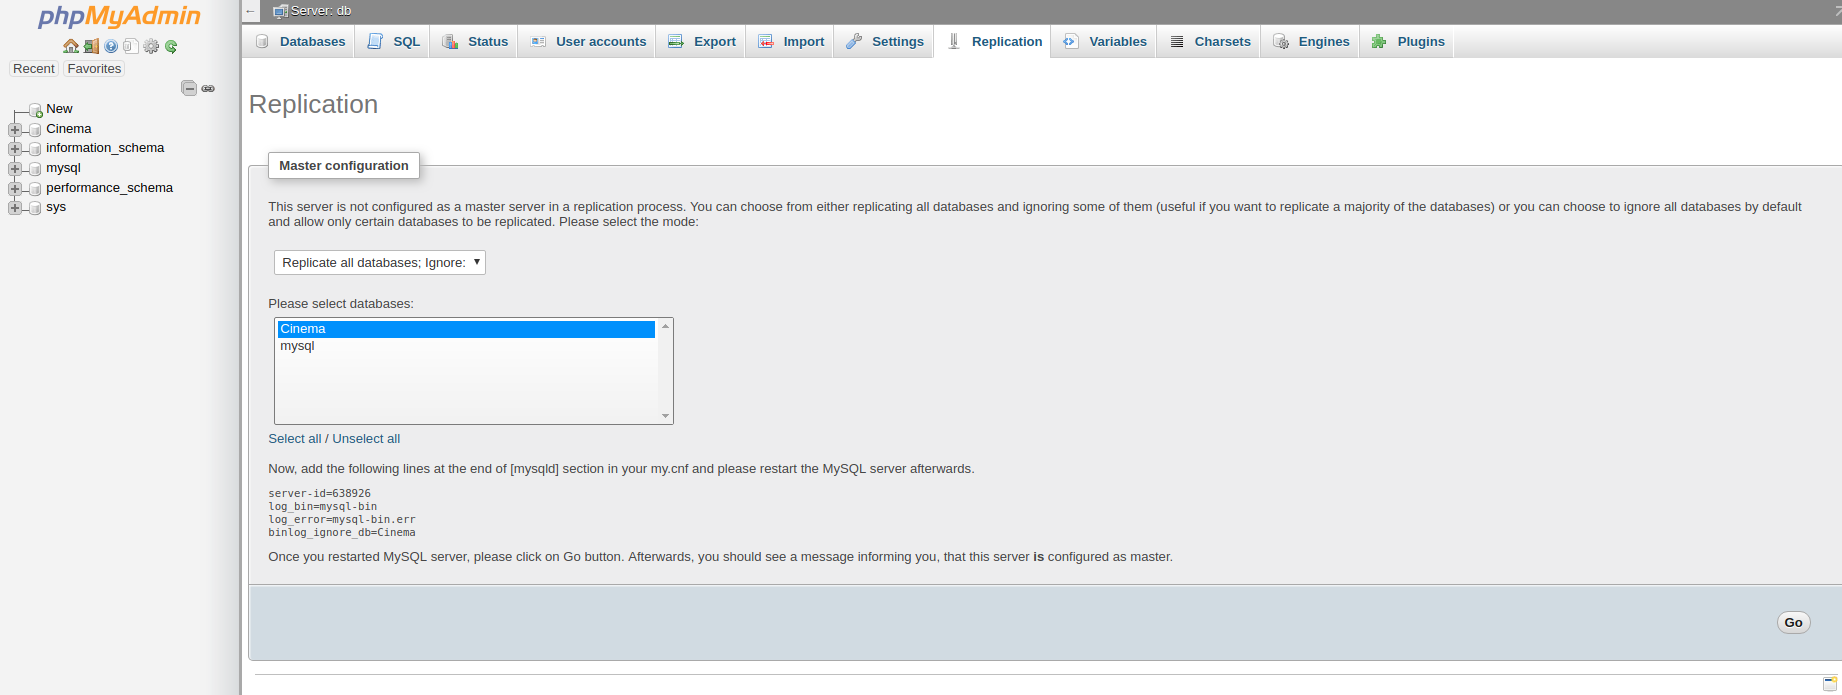
\includegraphics[width=1\linewidth]{rozdzial04/4.png}
	\caption{Konfiguracja serwera master w phpmyadmin}
	\label{fig:phpmyadmin2}
\end{figure}


By ustawić serwer jako slave, należy podać login i hasło do konta w węźle master, podać adres hosta oraz port, a następnie wcisnąć przycisk "GO".

\begin{figure} [H]
	\centering
	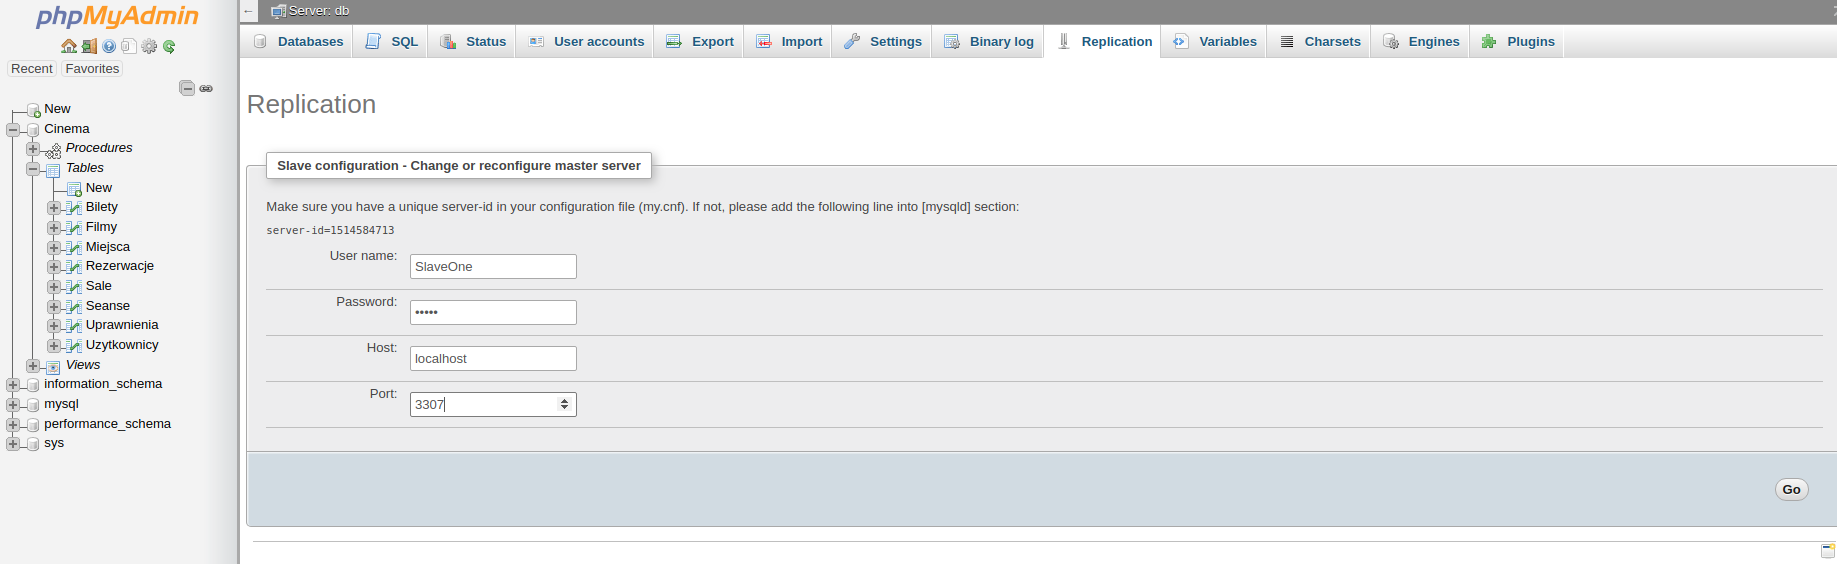
\includegraphics[width=1\linewidth]{rozdzial04/3.png}
	\caption{Konfiguracja serwera slave w phpmyadmin}
	\label{fig:phpmyadmin1}
\end{figure}

By dodać opóźnienie do węzła slave można z poziomu panelu phpmyadmin w zakładce SQL wydać komendę:

\lssetdef
\lstinputlisting[captionpos=b,caption={Konfiguracja opóźnienia dla węzła slave},label={lst:slave},basicstyle={\footnotesize\ttfamily}]{rozdzial04/slave.txt}

Dla takich danych opóźnienie wyniesie 120 sekund.

\section{Realizacja bazy danych}

\subsection{Tabele}

Tabele generowano za pomocą skryptów MySQL.

\begin{itemize}
	\item zdefiniowano klucze główne;
	\item zdefiniowano klucze obce;
	\item dodano ograniczenia jeżeli jakiś element nie może być pusty;
	\item tam gdzie to konieczne (login użytkownika, nazwa sali i nazwa uprawnień) dodano ograniczenia, aby dane te były unikalne w swoich tabelach;
	\item sprawdzanie czy podana liczba należy do przedziału wykorzystując słowo kluczowe \textit{CHECK} (pojemność sali musi się znajdować w przedziale od 20 do 450 miejsc);
	\item zabezpieczenie przed nadpisywaniem już wcześniej utworzonych tabel \textit{IF NOT EXISTS}.
\end{itemize}

\begin{figure} [H]
	\centering
	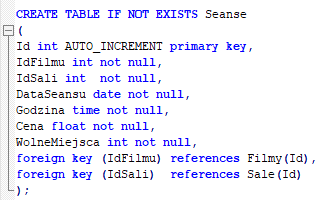
\includegraphics[width=0.6\linewidth]{rozdzial04/T_Seanse.png}
	\caption{Generowanie tabeli seansów}
	\label{fig:t_seanse}
\end{figure}

\begin{figure} [H]
	\centering
	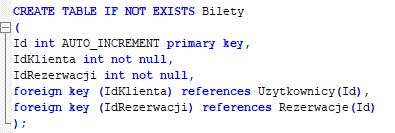
\includegraphics[width=0.6\linewidth]{rozdzial04/T_Bilety.png}
	\caption{Generowanie tabeli biletów - przykład użycia klucza głównego, kluczy obcych i ograniczenia "not null"}
	\label{fig:t_bilety}
\end{figure}

\begin{figure} [H]
	\centering
	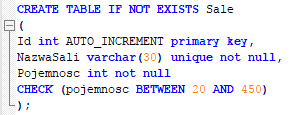
\includegraphics[width=0.5\linewidth]{rozdzial04/T_Sale.png}
	\caption{Generowanie tabeli sal - przykład użycia CHECK}
	\label{fig:t_sale}
\end{figure}

\subsection{Widoki}

\textbf{Utworzono trzy widoki:}

\begin{figure} [H]
	\centering
	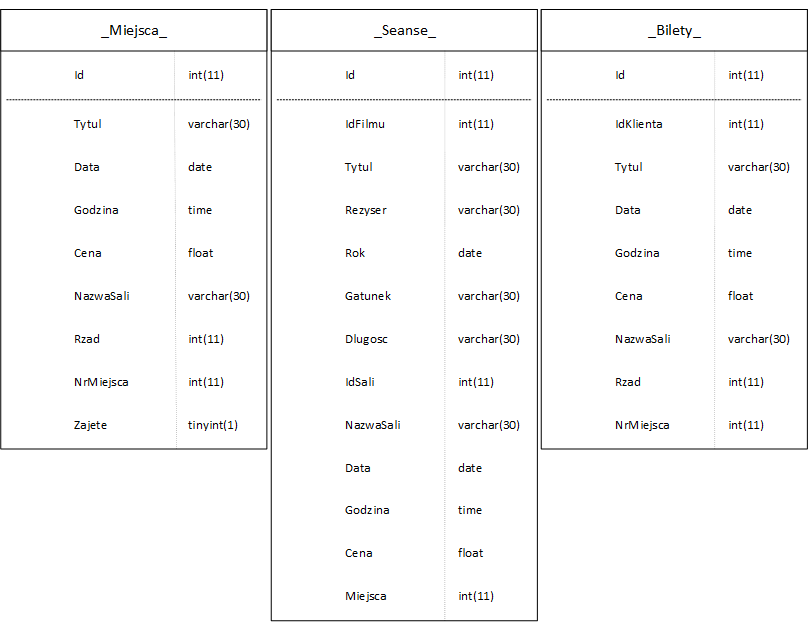
\includegraphics[width=0.8\linewidth]{rozdzial04/widoki.png}
	\caption{Wygenerowane widoki}
	\label{fig:views}
\end{figure}

\begin{itemize}
	\item \_Seanse\_ - rozszerza tabelę \textit{Seanse} o dodatkowe informacje o filmie, którego dotyczy seans i sali, na której seans zostanie wyświetlony;
	\item \_Miejsca\_ - rozszerza tabelę \textit{Rezerwacje} o informacje takie jak nazwa sali, rząd i numer miejsca.
	\item \_Bilety\_ - rozszerza tabelę \textit{Bilety} o informacje takie jak tytuł filmu, data, cena, nazwa sali, rząd oraz numer miejsca
\end{itemize}

\begin{figure} [H]
	\centering
	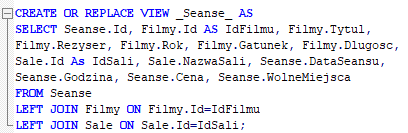
\includegraphics[width=0.6\linewidth]{rozdzial04/V_Seanse_.png}
	\caption{Generowanie widoku seansów}
	\label{fig:v_seanse}
\end{figure}

\begin{figure} [H]
	\centering
	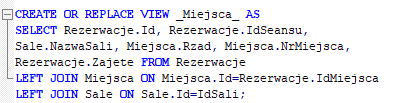
\includegraphics[width=0.6\linewidth]{rozdzial04/V_Miejsca_.png}
	\caption{Generowanie widoku Miejsc}
	\label{fig:v_miejsca}
\end{figure}

\subsection{Procedury}

Rysunek \ref{fig:procedury} przedstawia wszystkie procedury jakie zostały zaimplementowane. Natomiast na rysunku \ref{fig:p_DodajSeans} pokazana została jedna przykładowa procedura, która dodając seans dodaje również pulę miejsc równą pojemności sali, w której odbędzie się seans do tabeli \textit{Rezerwacje}.
\begin{figure} [H]
	\centering
	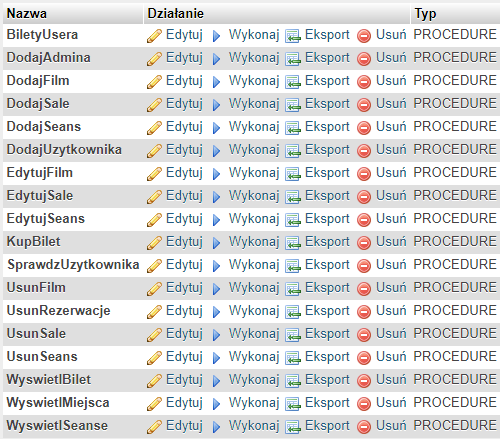
\includegraphics[width=0.7\linewidth]{rozdzial04/Procedury.png}
	\caption{Przykładowa procedura}
	\label{fig:procedury}
\end{figure}

\textbf{Opisy procedur:}
\begin{itemize}
	\item BiletyUsera - wyświetla wszystkie bilety które zostały zakupione przez konkretnego użytkownika;
	\item DodajAdmina - procedura pozwala na dodanie nowego użytkownika o uprawnieniach administratora;
	\item DodajFilm - pozwala na dodanie nowego filmu do filmoteki kina;
	\item DodajSale - pozwala dodać do bazy danych nowej sali kinowej;
	\item DodajSeans - umożliwia dodanie nowego seansu do oferty kina;
	\item DodajUzytkownika - procedura pozwala na dodanie nowego użytkownika o standardowych prawach zwykłego użytkownika;
	\item EdytujFilm - pozwala na zmienienie wszystkich informacji o filmie dostępnych w bazie;
	\item EdytujSale - pozwala na zmianę nazwy sali;
	\item EdytujSeans - pozwala modyfikować datę godzinę i cenę seansu;
	\item KupBilet - tworzy nowy rekord w tabeli Bilety, przypisuje go do konkretnego użytownika, oraz zmienia ilość wolnych miejsc na seansie, a w tabeli Rezerwacje oznacza miejsce jako zajęte;
	\item SprawdzUzytkownika - sprawdza czy użytkownik o podanym loginie i haśle istnieje w systemie;
	\item UsunFilm - usuwa film z filmoteki kina;
	\item UsunRezerwacje - usuwa wszystkie bilet, anuluje transakcję użytkownika, przywraca miejsce jako niezarezerwowane;
	\item UsunSale - usuwa sale i miejsca przypisane do sali, anuluje wszystkie seanse, które miały odbyć się na danej sali, i anuluje wszystkie bilety na te seanse;
	\item UsunSeans - anuluje seans i wszystkie bilety i rezerwacje na niego;
	\item WyswietlBilet - wyświetla informacje o bilecie o podanym id;
	\item WyswietlMiejsca - pokazuje wszystkie wolne miejsca na konkretny seans, korzystając z widoku \_Miejsca\_;
	\item WyswietlSeanse - wyświetla rozszerzone informacje o seansach z podanym filmem, korzystając z widoku \_Seanse\_.
\end{itemize}

\begin{figure} [H]
	\centering
	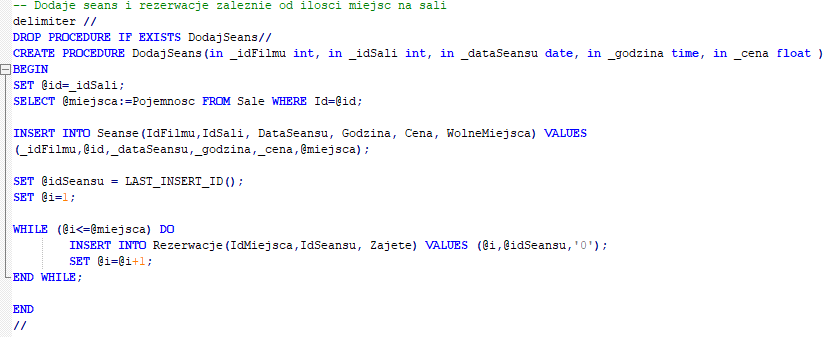
\includegraphics[width=1\linewidth]{rozdzial04/P_DodajSeans.png}
	\caption{Przykładowa procedura}
	\label{fig:p_DodajSeans}
\end{figure}

\section{Testowanie mechanizmów replikacji}
\label{chap:testReplikacji}

W projekcie użyta zostanie konfiguracja Master-Slave. Poniżej wypunktowane zostały wnioski z przeprowadzonych testów replikacji bazodanowej MySql.

\begin{itemize}
	\item Po skonfigurowaniu replikacji wymagane jest utworzenie bazy danych \textit{slave}, która posiada
	tą samą strukturę co \textit{master}
	\item Dane zawarte w bazie \textit{master} nie zostaną automatycznie skopiowane do bazy \textit{slave} po
	skonfigurowaniu replikacji. Należy ręcznie zsynchronizować dane w tabelach.
	\item W przypadku wyłączenia bazy danych \textit{slave} i modyfikacji bazy \textit{master} baza \textit{slave} zostanie
	zsynchronizowana po ponownym podłączeniu do sieci.
	\item \textit{Slave} – odczyt; \textit{master} – zapis, modyfikacja, usuwanie. Gdy \textit{slave} jest wyłączony zapytania
	GET są wysyłane do innego \textit{slave}, a w ostateczności \textit{mastera}. Gdy jest wyłączony \textit{master}
	można jedynie odczytywać dane z serwera. Natomiast na ten czas jakakolwiek modyfikacja
	danych jest niemożliwa.
	\item Od wersji\textit{ MySQL 5.7} możliwa jest replikacja Master-Slave z opóźnieniem. Domyślnie master natychmiastowo wysyła bin-log do węzłów typu \textit{slave}, jednak możliwe jest celowe wprowadzenie opóźnienia, np. w celu ochrony bazy danych przed poleceniem DROP, który wykonany na \textit{masterze}, usunie również bazę/ tabele na standardowych węzłach \textit{slave}. Odpowiednio duże opóźnienie daje możliwość na reakcję ze strony admina, tak aby w razie konieczności ocalić opóźniony węzeł.
\end{itemize}
	\chapter{Projekt i implementacja aplikacji klienckiej oraz REST API}

\section{Funkcje aplikacji}

%TODO: krótki opis

\subsection{Diagram przypadków użycia}

\begin{figure} [H]
	\centering
	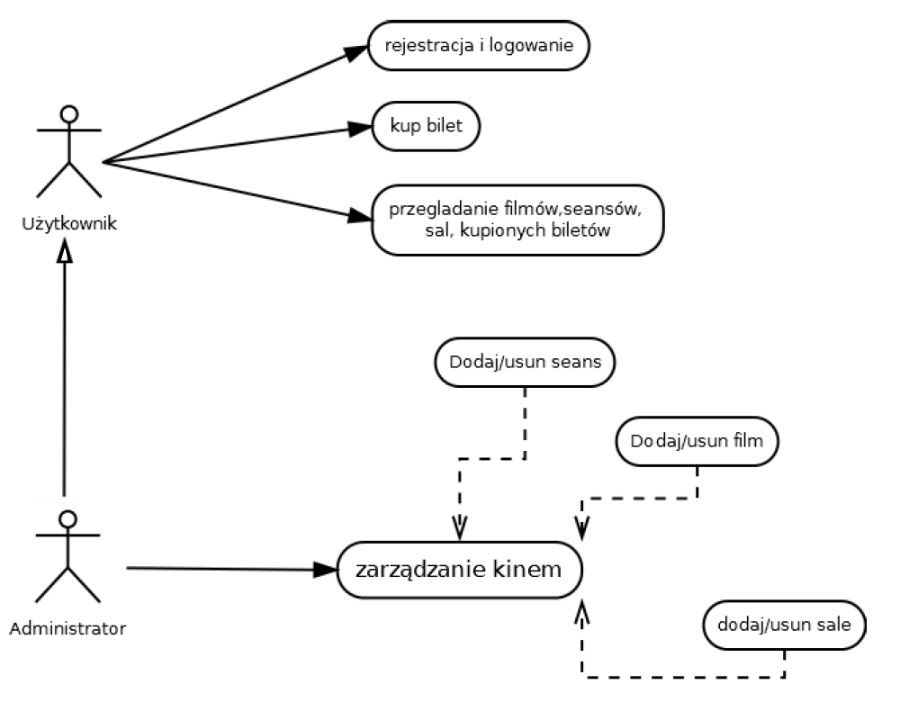
\includegraphics[width=0.6\linewidth]{rozdzial05/diagram.png}
	\caption{Diagram przypadków użycia}
	\label{fig:schem}
\end{figure}

Użytkownik:
\begin{itemize}
	\item tworzenie nowego konta (podanie loginu, hasła itp.);
	\item logowanie;
	\item przeglądanie filmów, seansów, kupionych biletów;
	\item kupowanie biletów.
\end{itemize}

Administrator:
\begin{itemize}
	\item te same funkcjonalności co użytkownik;
	\item dodawanie/usuwanie/edytowanie seansów;
	\item dodawanie/usuwanie/edytowanie filmów;
	\item dodawanie/usuwanie/edytowanie dostępnych sal.
\end{itemize}

\subsection{Scenariusz wybranych przypadków użycia}

W poniższych tabelach umieszczone zostały scenariusze wybranych przypadków użycia.

\begin{table}[H]
	\begin{tabularx}{\textwidth}{ |l|X| }
		\hline 
		Przypadek użycia & Rejestracja  \\ 
		\hline 
		Opis & Funkcja umożliwiająca założenie konta w systemie \\ 
		\hline 
		Warunki początkowe & Brak konta \\ 
		\hline 
		Warunki końcowe & System utworzył konto lub odrzucił żądanie  \\ 
		\hline 
		Przebieg podstawowy & 1. Użytkownik podaje swoje dane (login, hasło itp.) \\ 
		& 2. System sprawdza czy login nie jest zajęty \\
		& 3. Jeśli login jest wolny, skok do pkt 6. \\
		& 4. Wyświetlenie komunikatu o błędach \\
		& 5. Skok do pkt 1. \\
		& 6. Zakończenie rejestracji \\
		\hline 
	\end{tabularx} 
    \caption{Scenariusz rejestracji}
\label{tab:scen1}   
\end{table}

\begin{table}[H]
	\begin{tabularx}{\textwidth}{ |l|X| }
		\hline 
		Przypadek użycia & Logowanie  \\ 
		\hline 
		Opis & Funkcja umożliwiająca użytkownikom uzyskanie dostępu do systemu \\ 
		\hline 
		Warunki początkowe & Posiadanie własnego konta \\ 
		\hline 
		Warunki końcowe & System autoryzował, bądź odrzucił użytkownika  \\ 
		\hline 
		Przebieg podstawowy & 1. Użytkownik podaje swój login i hasło \\ 
		& 2. System wyszukuje użytkownika \\
		& 3. Jeśli użytkownik zostanie zweryfikowany, skok do pkt 6. \\
		& 4. Wyświetlenie komunikatu o błędach \\
		& 5. Skok do pkt 1. \\
		& 6. Zakończenie logowania \\
		\hline 
	\end{tabularx} 
	\caption{Scenariusz logowania}
	\label{tab:scen2}   
\end{table}

\begin{table}[H]
	\begin{tabularx}{\textwidth}{ |l|X| }
		\hline 
		Przypadek użycia & zarządzanie kinem  \\ 
		\hline 
		Opis & Funkcja umożliwiająca pracownikom zarządzanie kinem \\ 
		\hline 
		Warunki początkowe & Funkcja dostępna tylko dla zalogowanych pracowników \\ 
		\hline 
		Warunki końcowe & Dokonanie zmiany w systemie  \\ 
		\hline 
		Przebieg podstawowy & 1. Pracownik uruchamia aplikację zarządzania kinem \\ 
		& 2. Wywołanie odpowiedniego przypadku w zależności od wybranej akcji do wykonania \\
		& 3. Jeżeli wybrano "Dodanie filmu", wywołanie przypadku "Dodanie filmu". Skok do pkt 8. \\
		& 4. Jeżeli wybrano "Dodanie seansu", wywołanie przypadku "Dodanie seansu". Skok do pkt 8. \\
		& 5. Jeżeli wybrano "Usuwanie filmu", wywołanie przypadku "Usuwanie filmu". Skok do pkt 8. \\
		& 6. Jeżeli wybrano "Usuwanie seansu", wywołanie przypadku "Usuwanie seansu". Skok do pkt 8. \\
		& 7. Jeżeli wybrano "Dodawanie sali", wywołanie przypadku "Dodanie sali". Skok do pkt 8. \\
		& 8. Zakończenie procesu \\
		\hline
		Przebieg alternatywny & 1. Pracownik wchodzi na stronę zarządzania kinem. \\
		& 2. Wywołanie odpowiedniego przypadku w zależności od wybranej akcji do wykonania \\
		& 3. Pracownik wylogował się z systemu \\
		& 4. zakończenie procesu. \\
		\hline 
	\end{tabularx} 
	\caption{Scenariusz zarządzania kinem}
	\label{tab:scen3}   
\end{table}

\section{Realizacja wybranych funkcjonalności aplikacji}

Aplikacja internetowa powstała z wykorzystaniem platformy programistycznej Angular 2. Jest to framework odpowiedzialny za tworzenia aplikacji po stronie klienta. Do zaprogramowania części funkcjonalnej aplikacji wykorzystuje on TypeScript czyli wolny i otwartoźródłowy język programowania stworzony przez firmę Microsoft jako nadzbiór języka JavaScript. Umożliwia on opcjonalne statyczne typowanie oraz programowanie zorientowane obiektowo oparte na klasach. TypeScript jest nadzbiorem JavaScript, a więc potencjalnie każdy program napisany w języku JavaScript jest poprawnym programem TypeScript. Aplikacje napisane w TypeScript kompilują się bezpośrednio do języka JavaScript. Poniżej znajdują się przykładowe fragmenty kodu napisane w tym języku odpowiedzialne za komunikację z API bazy danych.  

\lssetdef
\lstinputlisting[captionpos=b,caption={Implementacja funkcji GET po stronie aplikacji},label={lst:Get},basicstyle={\footnotesize\ttfamily}]{rozdzial05/GET.txt}

\lstinputlisting[captionpos=b,caption={Implementacja funkcji POST po stronie aplikacji},label={lst:Post},basicstyle={\footnotesize\ttfamily}]{rozdzial05/POST.txt}

\subsection{Interfejs aplikacji}

Aplikacja została napisana tak aby blokować widok niedozwolonych operacji jeśli użytkownik nie ma odpowiednich uprawnień. Poniżej znajdują się zrzuty ekranu widoku interfejsu z konta administracyjnego. 

\begin{figure} [H]
	\centering
	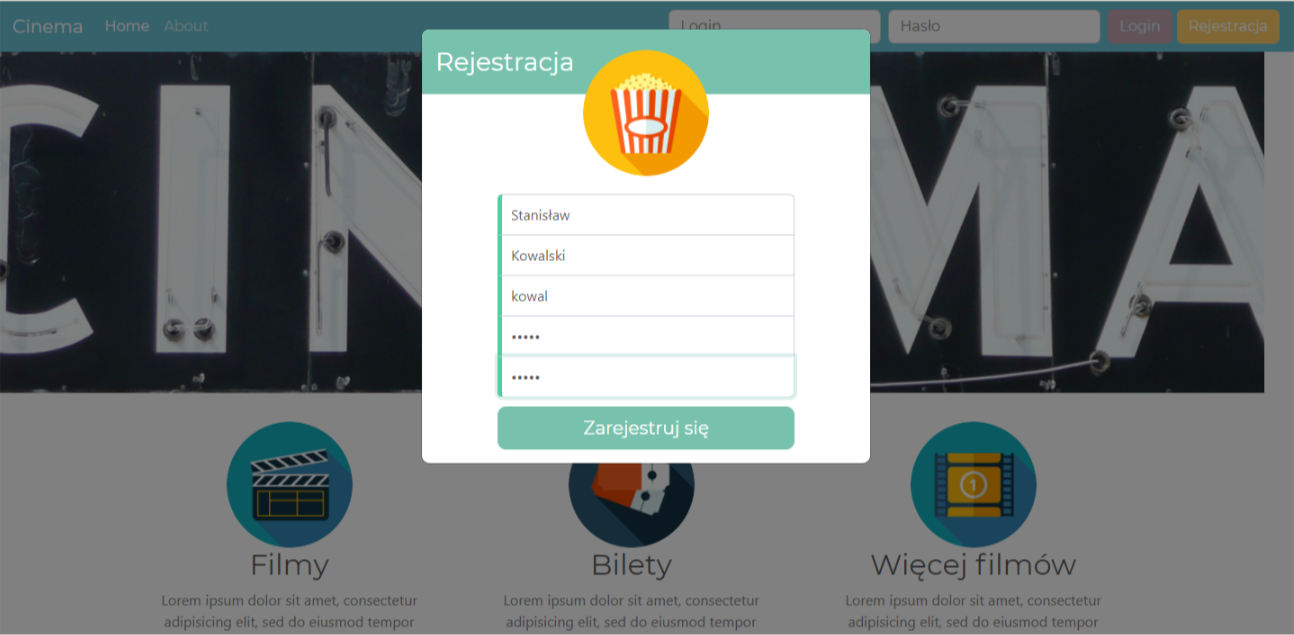
\includegraphics[width=1\linewidth]{rozdzial05/interfejs/rejestracja.png}
	\caption{Rejestracja użytkownika}
	\label{fig:screen1}
\end{figure}


\begin{figure} [H]
	\centering
	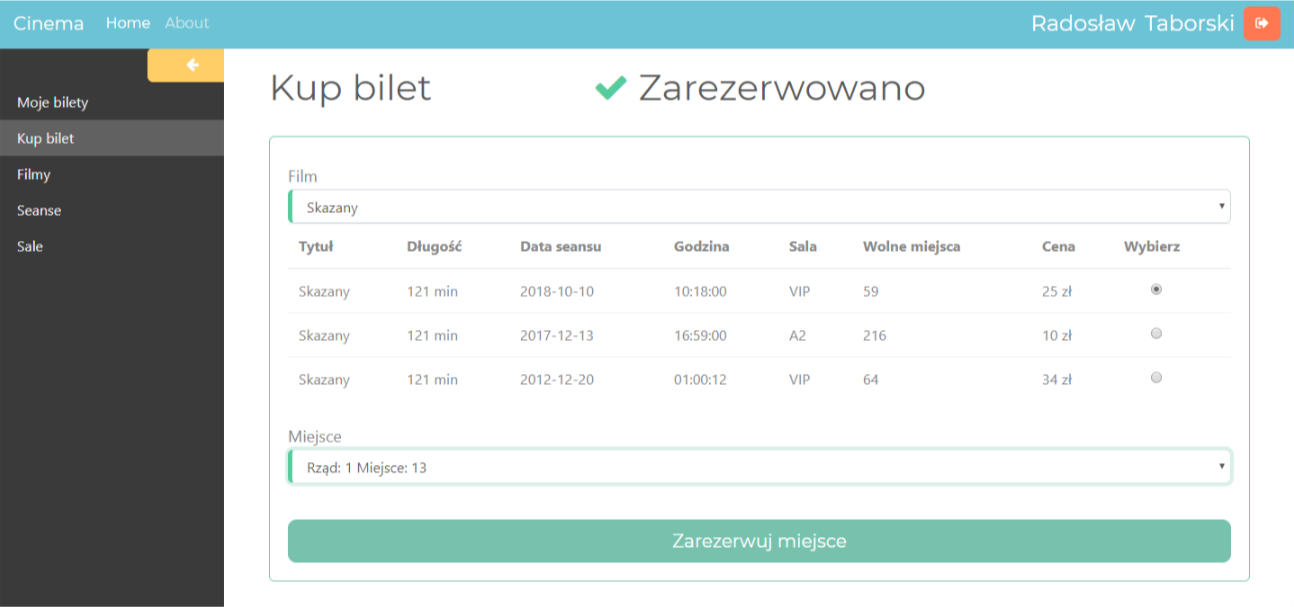
\includegraphics[width=1\linewidth]{rozdzial05/interfejs/kupBilet.png}
	\caption{Rezerwacja biletów}
	\label{fig:screen2}
\end{figure}

\begin{figure} [H]
	\centering
	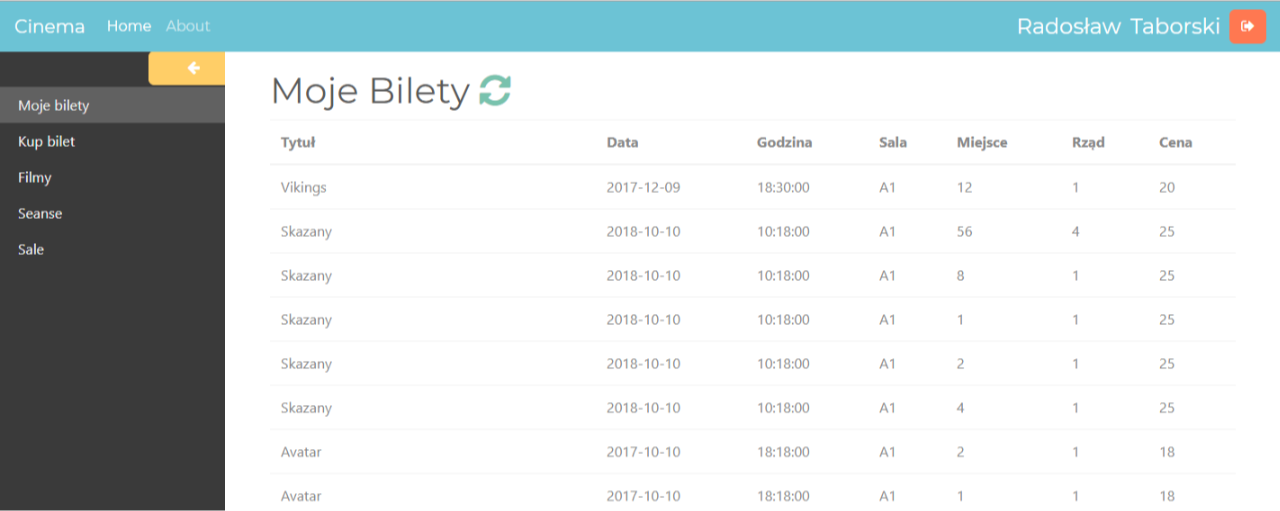
\includegraphics[width=1\linewidth]{rozdzial05/interfejs/mojeBilety.png}
	\caption{Widok biletów zarezerwowanych przez użytkownika}
	\label{fig:screen3}
\end{figure}

\begin{figure} [H]
	\centering
	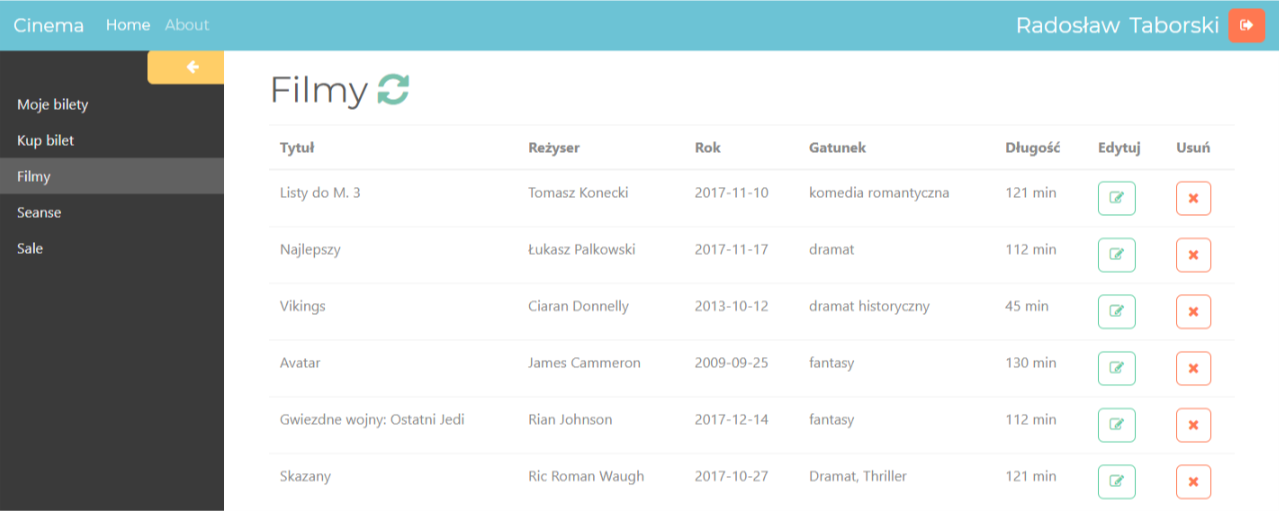
\includegraphics[width=1\linewidth]{rozdzial05/interfejs/filmy.png}
	\caption{Widok filmów dostępnych w kinie}
	\label{fig:screen4}
\end{figure}

\begin{figure} [H]
	\centering
	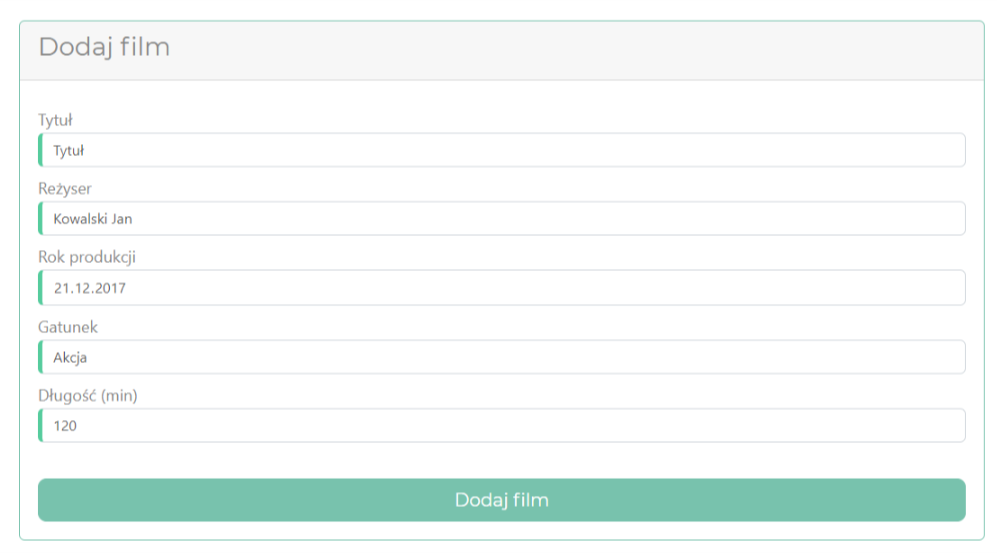
\includegraphics[width=1\linewidth]{rozdzial05/interfejs/dadajFilm.png}
	\caption{Dodawanie nowego filmu}
	\label{fig:screen5}
\end{figure}

\begin{figure} [H]
	\centering
	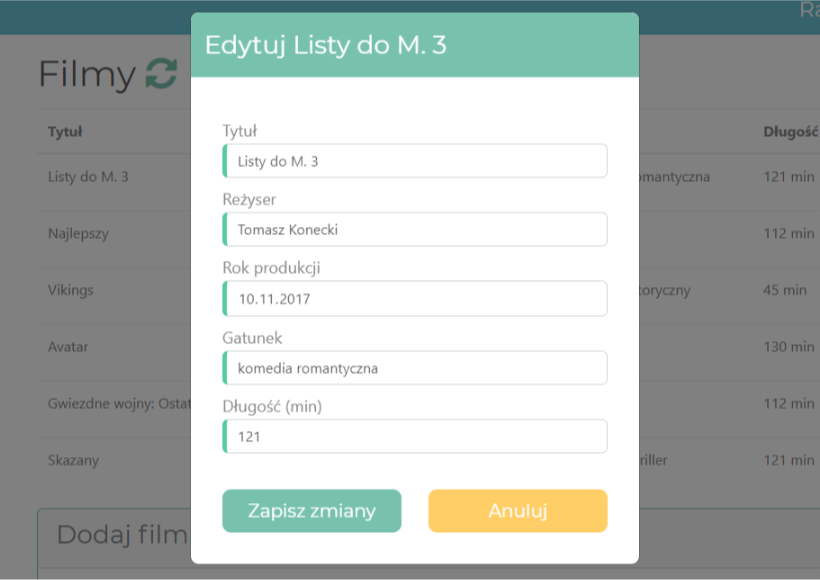
\includegraphics[width=1\linewidth]{rozdzial05/interfejs/edytujFilm.png}
	\caption{Edycja filmu}
	\label{fig:screen6}
\end{figure}

\begin{figure} [H]
	\centering
	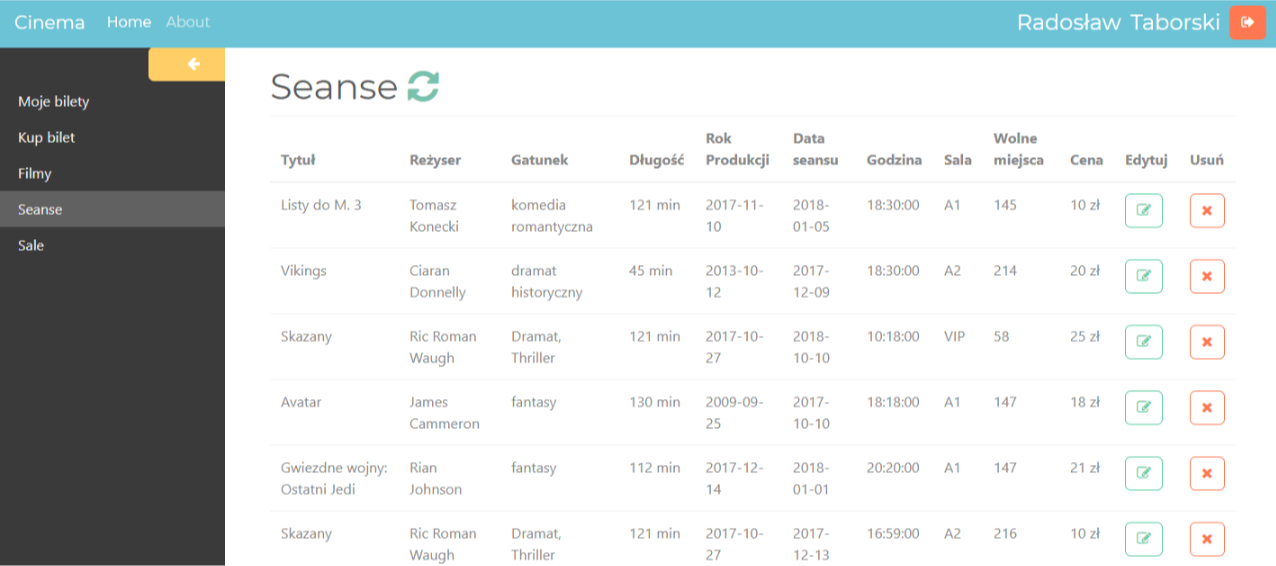
\includegraphics[width=1\linewidth]{rozdzial05/interfejs/seanse.png}
	\caption{Widok seansów dostępnych w kinie}
	\label{fig:screen7}
\end{figure}

\begin{figure} [H]
	\centering
	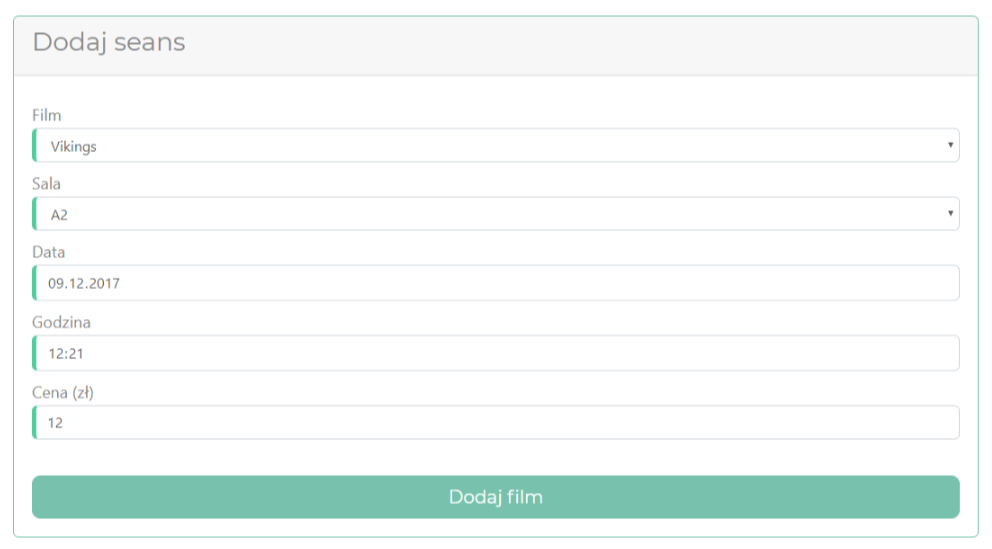
\includegraphics[width=1\linewidth]{rozdzial05/interfejs/dodajSeans.png}
	\caption{Dodawanie seansu}
	\label{fig:screen8}
\end{figure}

\begin{figure} [H]
	\centering
	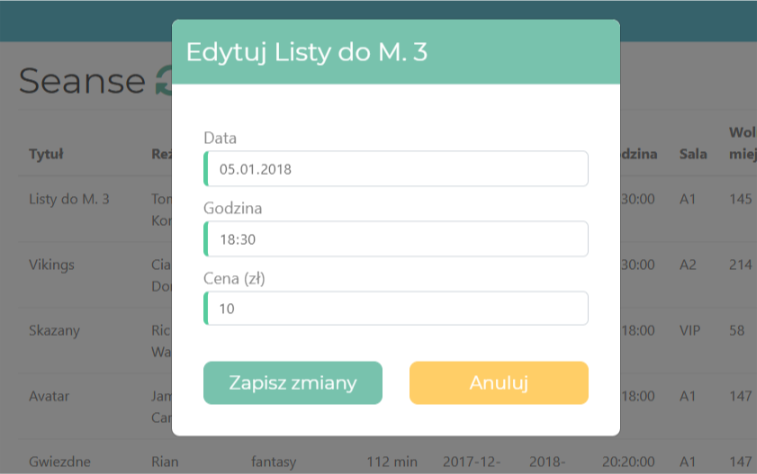
\includegraphics[width=1\linewidth]{rozdzial05/interfejs/edytujSeans.png}
	\caption{Edycja seansu}
	\label{fig:screen9}
\end{figure}

\begin{figure} [H]
	\centering
	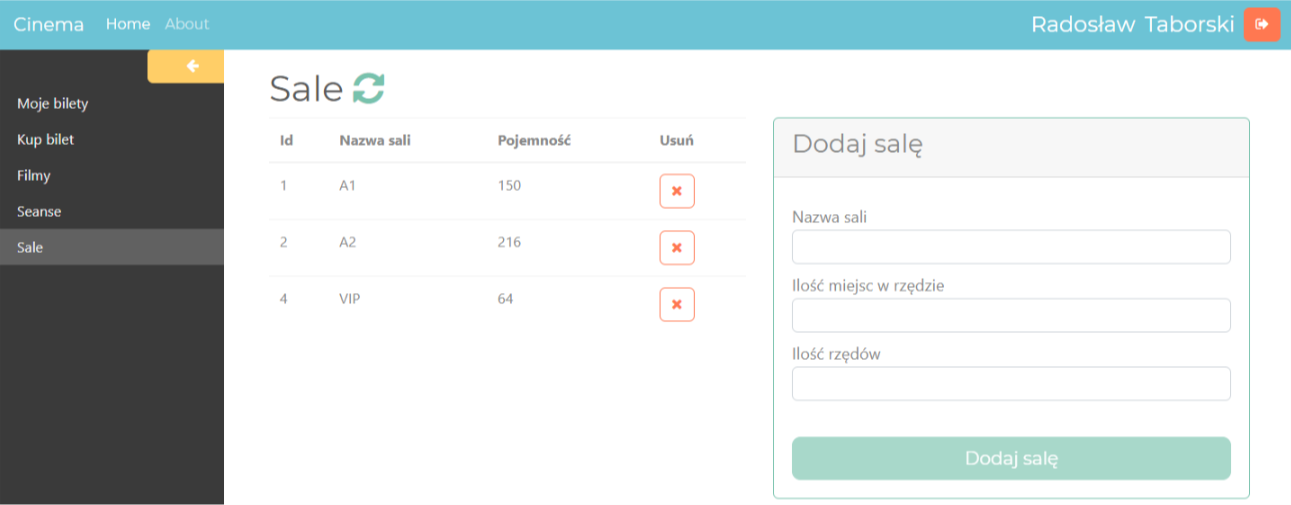
\includegraphics[width=1\linewidth]{rozdzial05/interfejs/sale.png}
	\caption{Widok sal dostępnych w kinie}
	\label{fig:screen10}
\end{figure}

Aplikacja również informuje o błędach z łącznością z serwerem (rysunek \ref{fig:alert2}) oraz o podaniu błędnego loginu lub hasła (rysunek \ref{fig:alert1})

\begin{figure} [H]
	\centering
	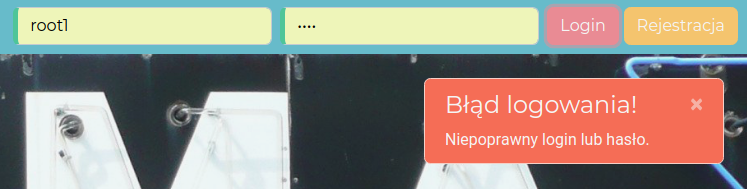
\includegraphics[width=1\linewidth]{rozdzial05/interfejs/alert1.png}
	\caption{Podanie błędnego loginu i hasła}
	\label{fig:alert1}
\end{figure}
		
\begin{figure} [H]
	\centering
	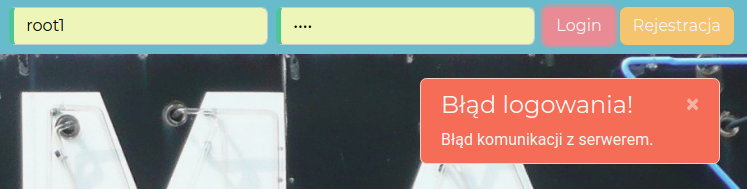
\includegraphics[width=1\linewidth]{rozdzial05/interfejs/alert2.png}
	\caption{Błąd komunikacji z serwerem}
	\label{fig:alert2}
\end{figure}

\section{Realizacja REST API}

REST (ang. Representational State Transfer) jest wzorcem narzucającym dobre praktyki tworzenia architektury aplikacji rozproszonych. RESTful Webservices (inaczej RESTful web API) jest usługą sieciową zaimplementowaną na bazie protokołu HTTP i głównych zasad wzorca REST. Ważnym założeniem REST jest istnienie zasobów (ang. resources) jako źródeł danych a także żądana akcja. API aplikacji zostało stworzone w postaci skryptu w PHP.

\begin{table}[H]
\centering

\label{restApi}
\begin{tabular}{|l|l|l|}
\hline
\textbf{zasób}                               & \textbf{metoda} & \textbf{zastosowanie}                \\ \hline
http://90.156.81.49:81/cinemaapi.php/filmy   & GET             & zostanie zwrócona lista filmów       \\ \hline
http://90.156.81.49:81/cinemaapi.php/filmy/1 & GET             & zostanie zwrócony film o id równym 1 \\ \hline
http://90.156.81.49:81/cinemaapi.php/film    & PUT             & dodanie nowego filmu                 \\ \hline
http://90.156.81.49:81/cinemaapi.php/film/1  & POST            & edycja filmu o id równym 1           \\ \hline
http://90.156.81.49:81/cinemaapi.php/film/1  & DELETE          & usunięcie filmu o id równym 1        \\ \hline
\end{tabular}
\caption{Przykładowe zastosowanie REST API}
\end{table}

Poniżej znajdują się fragmenty skryptu odpowiedzialnego za obsługę zapytań.

\lstinputlisting[captionpos=b,caption={Skrypt PHP API aplikacji},label={lst:api},basicstyle={\footnotesize\ttfamily}]{rozdzial05/cinemaApi.txt}

\lstinputlisting[captionpos=b,caption={Skrypt PHP obsługujący zapytania GET},label={lst:php},basicstyle={\footnotesize\ttfamily}]{rozdzial05/getApi.txt}
	\chapter{Wdrożenie i testowanie aplikacji klienckiej}

\section{Wdrożenie aplikacji klienckiej}
\subsection{Konfigurowanie środowiska wirtualnego}
Aplikacja kliencka została stworzona jako aplikacja webowa z wykorzystaniem platformy programistycznej \textit{Angular 2}. By móc skorzystać z tego frameworku należy odpowiednio skonfigurować środowisko.

W pierwszej kolejności wymagane jest zainstalowanie środowiska uruchomieniowego Node.js, które zaprojektowane zostało do tworzenia wysoce skalowalnych aplikacji internetowych, szczególnie pod kątem serwisów www napisanych w języku JavaScript. \'Srodowisko to jest dostępne do pobrania ze strony internetowej node.js [6]. Bądź też jak to zostało wykonane w ramach projektu na systemie operacyjnym Ubuntu 16.04 poprzez komendy na listingu~\ref{lst:node}.

\lssetdef
\lstinputlisting[captionpos=b,caption={Instalacja Node.js w systemie operacyjnym Ubuntu 16.04},label={lst:node},basicstyle={\footnotesize\ttfamily}]{rozdzial06/node.txt}

Kolejnym krokiem jest instalacja Angular-CLI poprzez komendy z listingu~\ref{lst:angular}

\lssetdef
\lstinputlisting[captionpos=b,caption={Instalacja Angular-CLI w systemie operacyjnym Ubuntu 16.04},label={lst:angular},basicstyle={\footnotesize\ttfamily}]{rozdzial06/angular2.txt}

Tak przygotowane środowisko umożliwia już uruchomienie aplikacji klienckiej. By uruchomić aplikację na \textit{localhost:4200} w przeglądarce internetowej wystarczy będąc w katalogu z aplikacją wydać polecenia z listingu~\ref{lst:localhost}. W tym przypadku polecenie pierwsze odpowiedzialne jest za przebudowanie projektu i wymagane jest jedynie w przypadku dodania do projektów nowych pakietów.

\lssetdef
\lstinputlisting[captionpos=b,caption={Uruchomienie aplikacji na localhost:4200 16.04},label={lst:localhost},basicstyle={\footnotesize\ttfamily}]{rozdzial06/localhost.txt}

\subsection{Zmiana domyślnego portu działania aplikacji}
Zmiana portu umożliwia uruchomienie projektu na serwerze, tak by mógł być widoczny bądź w sieci lokalnej bądź globalnie. \\

W tym celu w głównym katalogu aplikacji umieszczony został plik \textit{server.js} oraz katalog \textit{server}, w którym z kolei umieszczony został plik \textit{api.js}\\

Na listingu~\ref{lst:server} przedstawiona została zawartość pliku server.js. Numer portu na jaki został przekierowany serwis ustawiony został w 29 linii pliku.

\lssetdef
\lstinputlisting[captionpos=b,caption={Zawartość pliku server.js},label={lst:server},basicstyle={\footnotesize\ttfamily}]{rozdzial06/server.txt}

\lssetdef
\lstinputlisting[captionpos=b,caption={Zawartość pliku api.js},label={lst:api},basicstyle={\footnotesize\ttfamily}]{rozdzial06/api.txt}

Po utworzeniu tych plików uruchomienie aplikacji klienckiej na nowym porcie odbywa się poprzez komendę z listingu~{lst:run}.

\lssetdef
\lstinputlisting[captionpos=b,caption={Uruchomienie aplikacji klienckiej na własnym porcie},label={lst:run},basicstyle={\footnotesize\ttfamily}]{rozdzial06/run.txt}

\subsection{Wdrożenie API REST-owego}
Do poprawnego działania aplikacji potrzebne jest również API REST-owe pośredniczące w komunikacji aplikacji klienckiej z rozproszoną bazą danych. Podczas wdrażania projektu na systemie operacyjnym Ubuntu 16.04, API zostało umieszczone na serwerze HTTP- \textit{APACHE2}.

\section{Testy działania aplikacji}

W tej części zostały zamieszczone obrazy działania wprowadzonej aplikacji, a tym samym również poprawność działania replikacji między węzłami rozproszonej bazy danych. Aplikacja działa poprawnie i zgodnie z przewidywaniami. \\

Tak jak to już zostało wspomniane w podrozdziale \ref{chap:testReplikacji}, by replikacja mogła przebiegać prawidłowo, bazy na węzłach \textit{slave} muszą być spójne z bazą na węźle \textit{master}, a co z tego poniekąd wynika bazy na wezłach \textit{slave} muszą być utworzone i muszą posiadać taką samą strukturę tabel.

\subsection{Dodawanie rekordu do rozproszonej bazy danych}
Na rysunkach od \ref{fig:addFilm} do \ref{fig:endAddFilm} zademonstrowane zostało działanie replikacji na przykładzie dodawania filmu do bazy z poziomu aplikacji webowej.\\

Na rysunku \ref{fig:addFilm} wpisane zostały dane przykładowego filmu, a po naciśnięciu przycisku 'Dodaj film' aplikacja poprzez API REST łączy się z węzłem master rozproszonej bazy danych, gdyż wprowadzana będzie modyfikacja, a następnie dodaje dane do tabeli Filmy (rysunek \ref{fig:FilmMaster}) dzięki procedurze SQL 'DodajFilm'. Wykonana procedura zostaje replikowana do wszystkich węzłów Slave. Tabela Filmy dla wybranego węzła Slave na porcie 8083 została pokazana na rysunku \ref{fig:FilmSlave}. Z węzła Slave również odczytywane są dane poprzez aplikację kliencką, a poprawnie odczytane dane z takiego węzła zostały przedstawione na rysunku \ref{fig:endAddFilm}.

\begin{figure} [H]
	\centering
	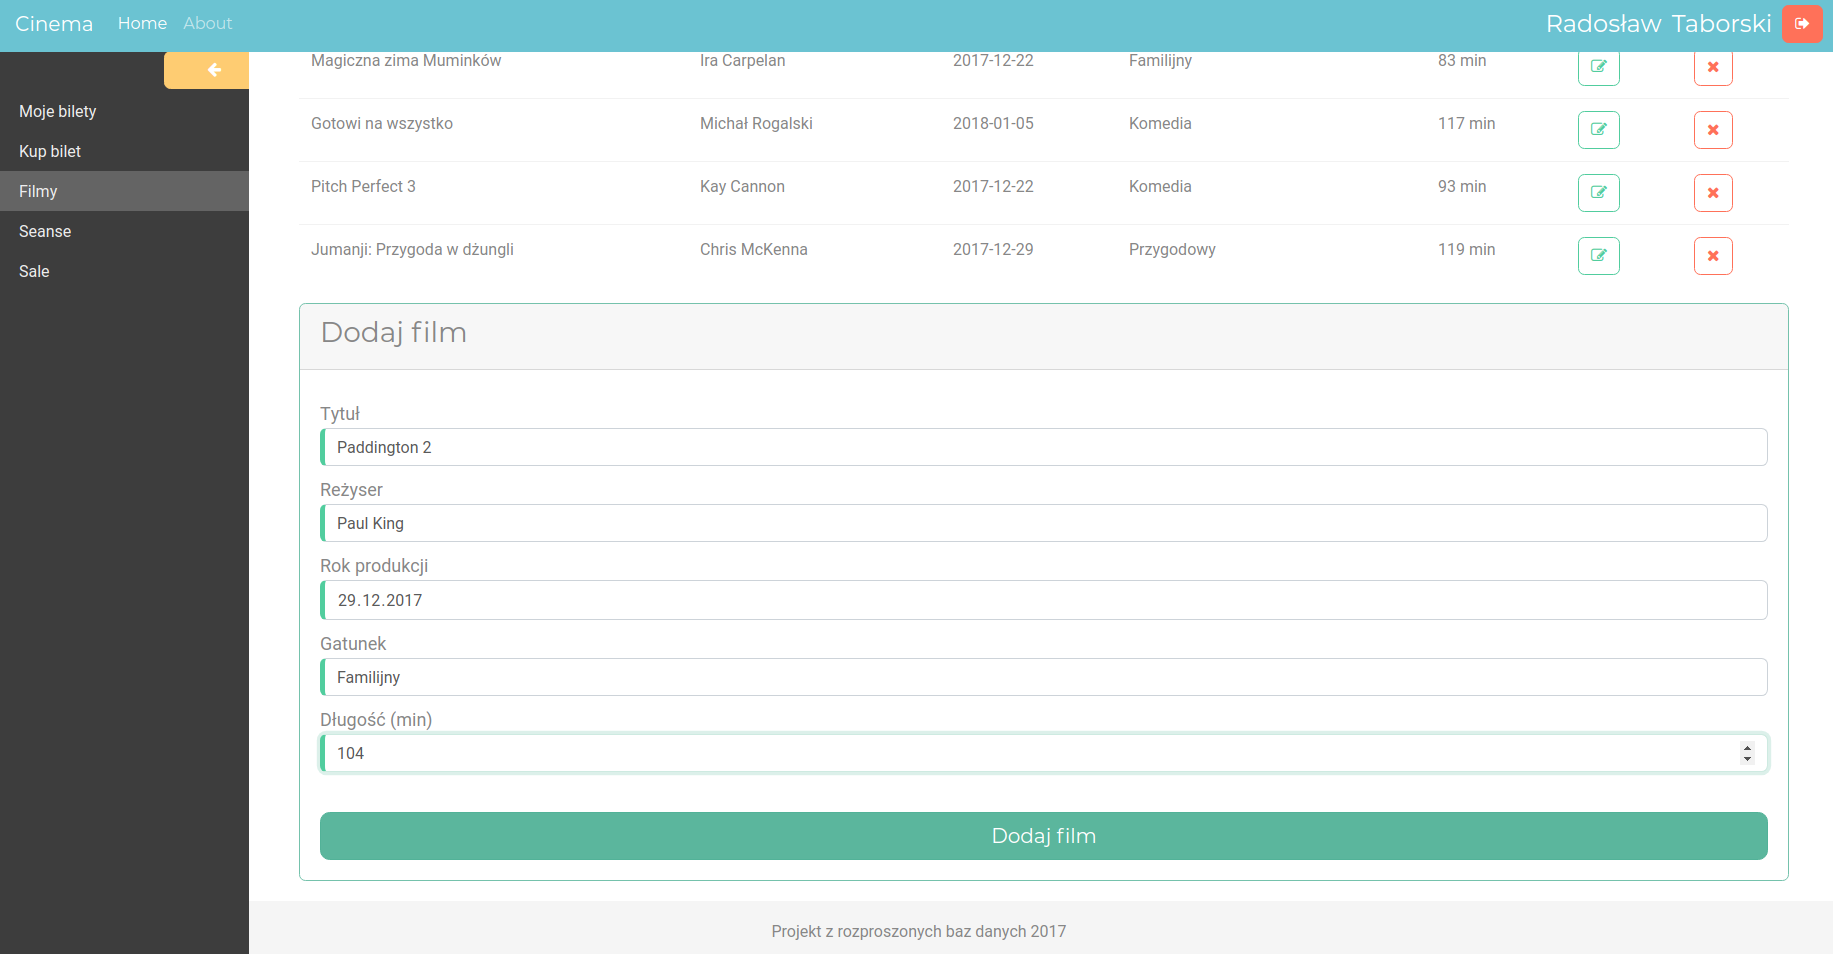
\includegraphics[width=1\linewidth]{rozdzial06/5.png}
	\caption{Dodawanie nowego filmu poprzez aplikację}
	\label{fig:addFilm}
\end{figure}

\begin{figure} [H]
	\centering
	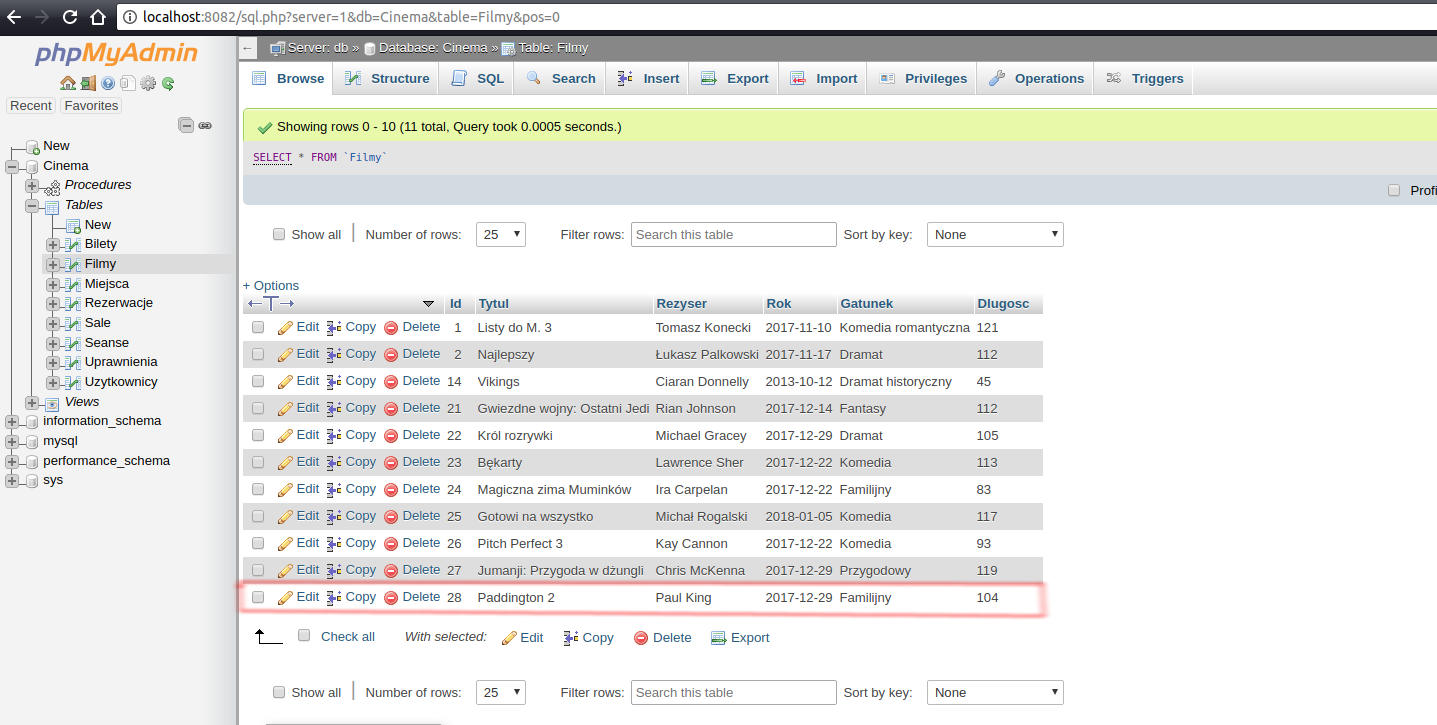
\includegraphics[width=1\linewidth]{rozdzial06/7.png}
	\caption{Tabela Filmy na węźle \textit{master} o porcie 8082}
	\label{fig:FilmMaster}
\end{figure}

\begin{figure} [H]
	\centering
	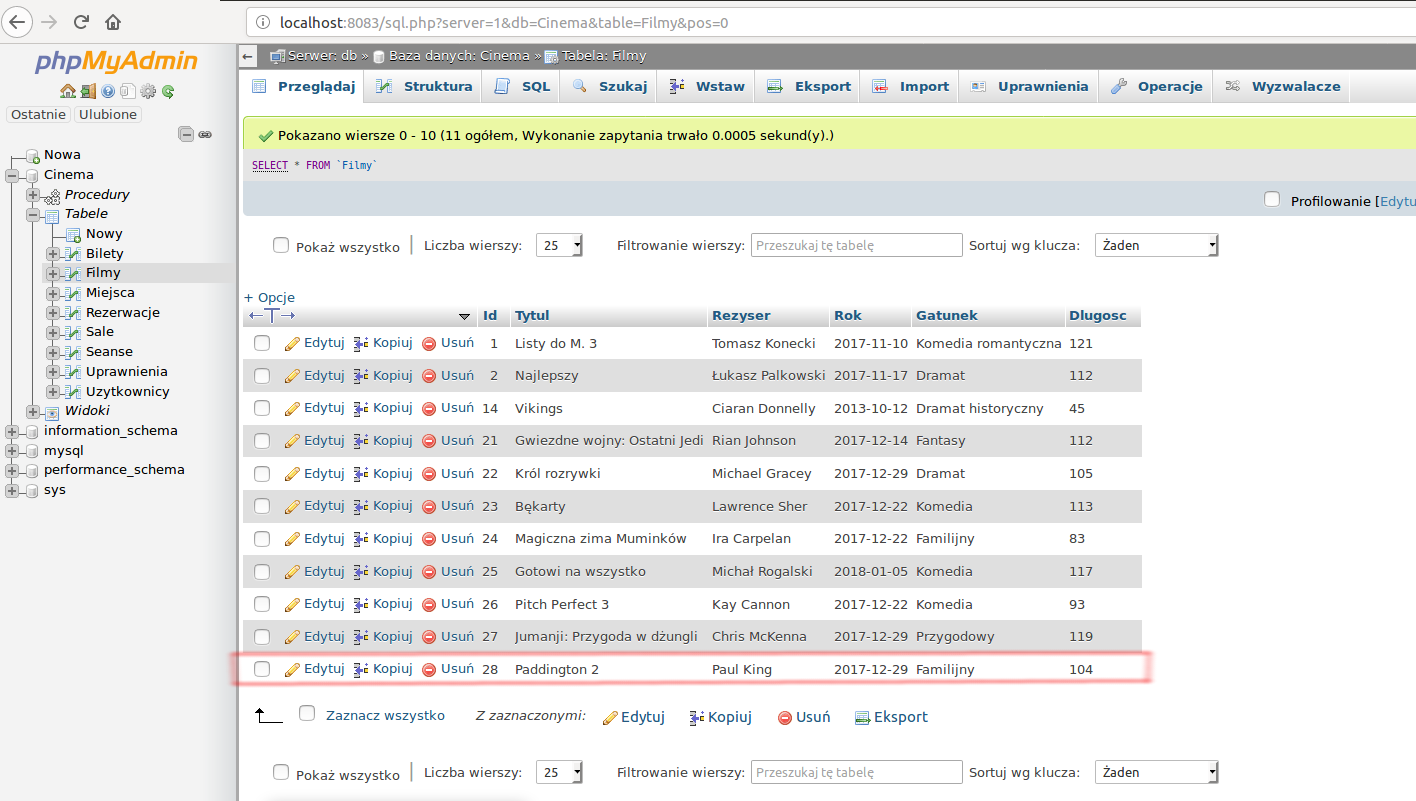
\includegraphics[width=1\linewidth]{rozdzial06/8.png}
	\caption{Tabela Filmy na węźle \textit{slave1} o porcie 8083}
	\label{fig:FilmSlave}
\end{figure}

\begin{figure} [H]
	\centering
	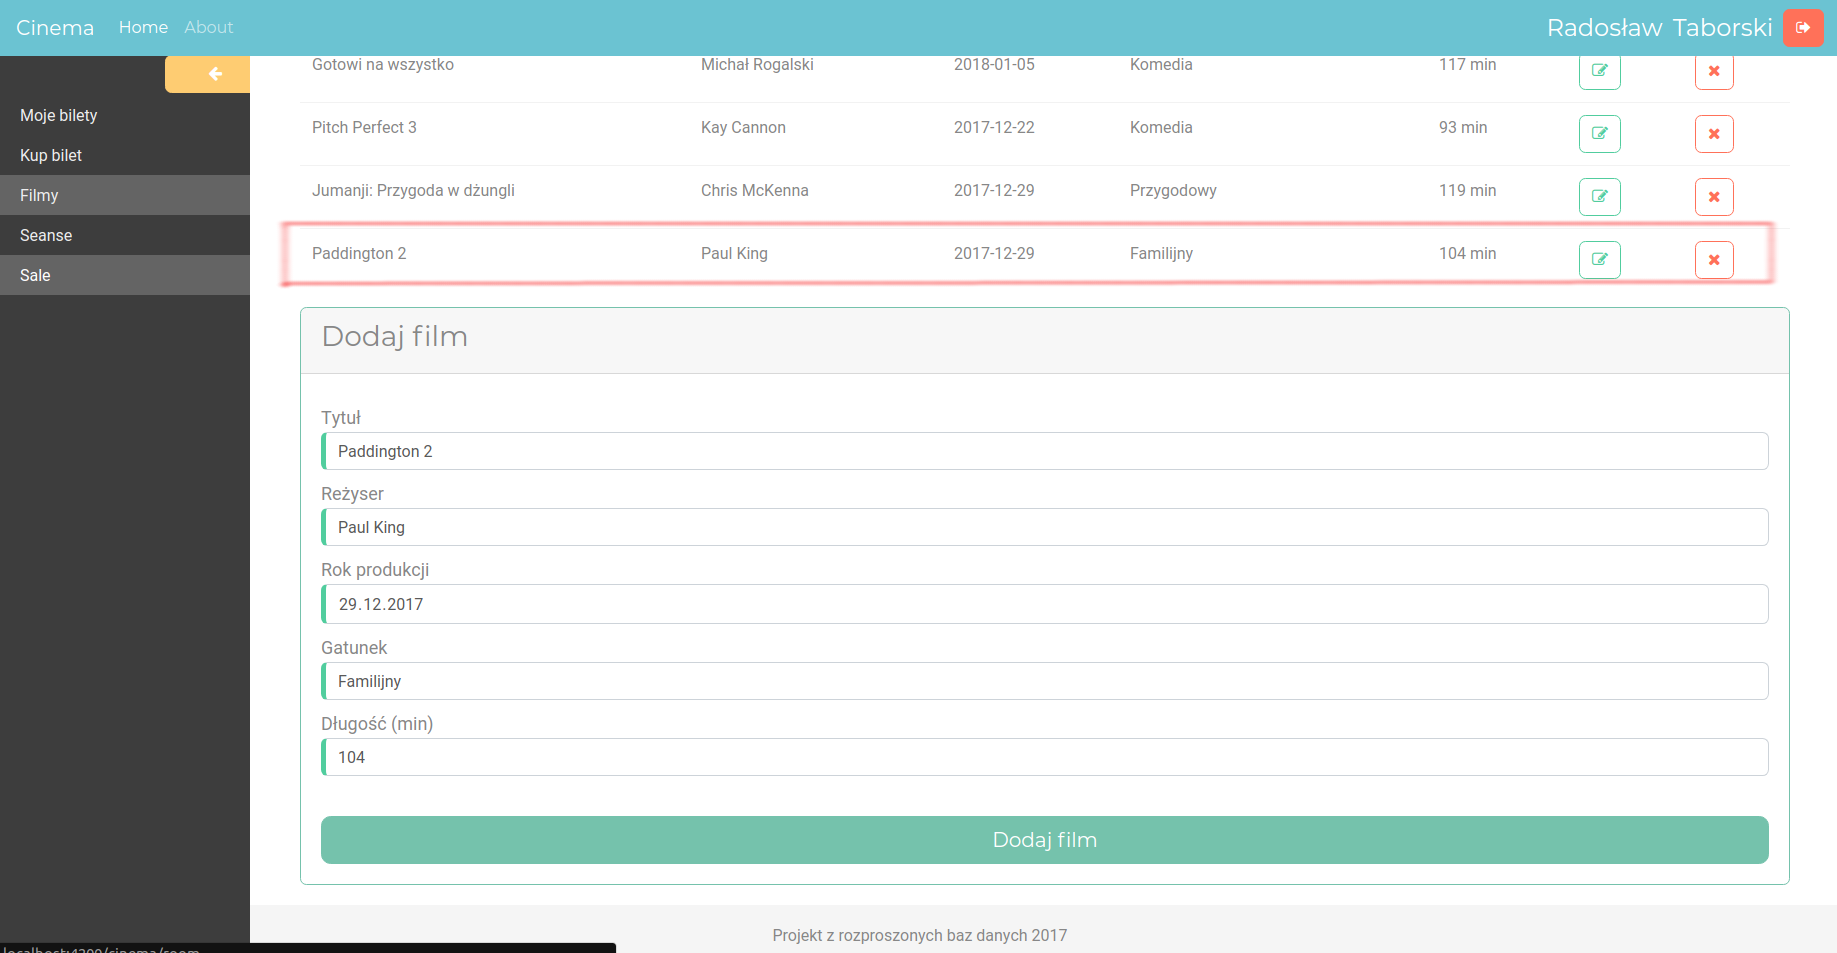
\includegraphics[width=1\linewidth]{rozdzial06/6.png}
	\caption{Nowy film wyświetlany w aplikacji}
	\label{fig:endAddFilm}
\end{figure}

\subsection{Usuwanie rekordu z rozproszonej bazy danych}

Na rysunkach od \ref{fig:removeFilm} do \ref{fig:endRemoveFilm} zademonstrowane zostało działanie replikacji na przykładzie dodawania filmu do bazy z poziomu aplikacji webowej.\\

Na rysunku \ref{fig:removeFilm} przedstawione zostały filmy znajdujące się w bazie danych wyświetlane poprzez aplikację kliencką. Będąc zalogowanym na konto administratorskie można usunąć film znajdujący się w bazie. Można tego dokonać poprzez kliknięcie czerwonego przycisku "X" obok wybranego filmu. Aplikacja wtedy łączy się poprzez API REST z węzłem master rozproszonej bazy danych, gdyż wprowadzana będzie modyfikacja, a następnie usunięty zostaje wybrany film z tabeli Filmy (rysunek \ref{fig:FilmMasterRemove}), dzięki procedurze SQL 'UsunFilm'. Wykonana procedura zostaje zreplikowana do wszystkich węzłów Slave. Tabela Filmy dla wybranego węzła Slave na porcie 8083 została pokazana na rysunku \ref{fig:FilmSlaveRemove}. Z węzła Slave również odczytywane są dane poprzez aplikację kliencką, a poprawnie odczytane dane z takiego węzła zostały przedstawione na rysunku \ref{fig:endRemoveFilm}. W przedstawionym przykładzie usunięty został film, który na rysunku~\ref{fig:FilmMaster} widoczny jest pod ID = 27. Jest to film o nazwie \textit{Jumanji: Przygoda w dżungli}.

\begin{figure} [H]
	\centering
	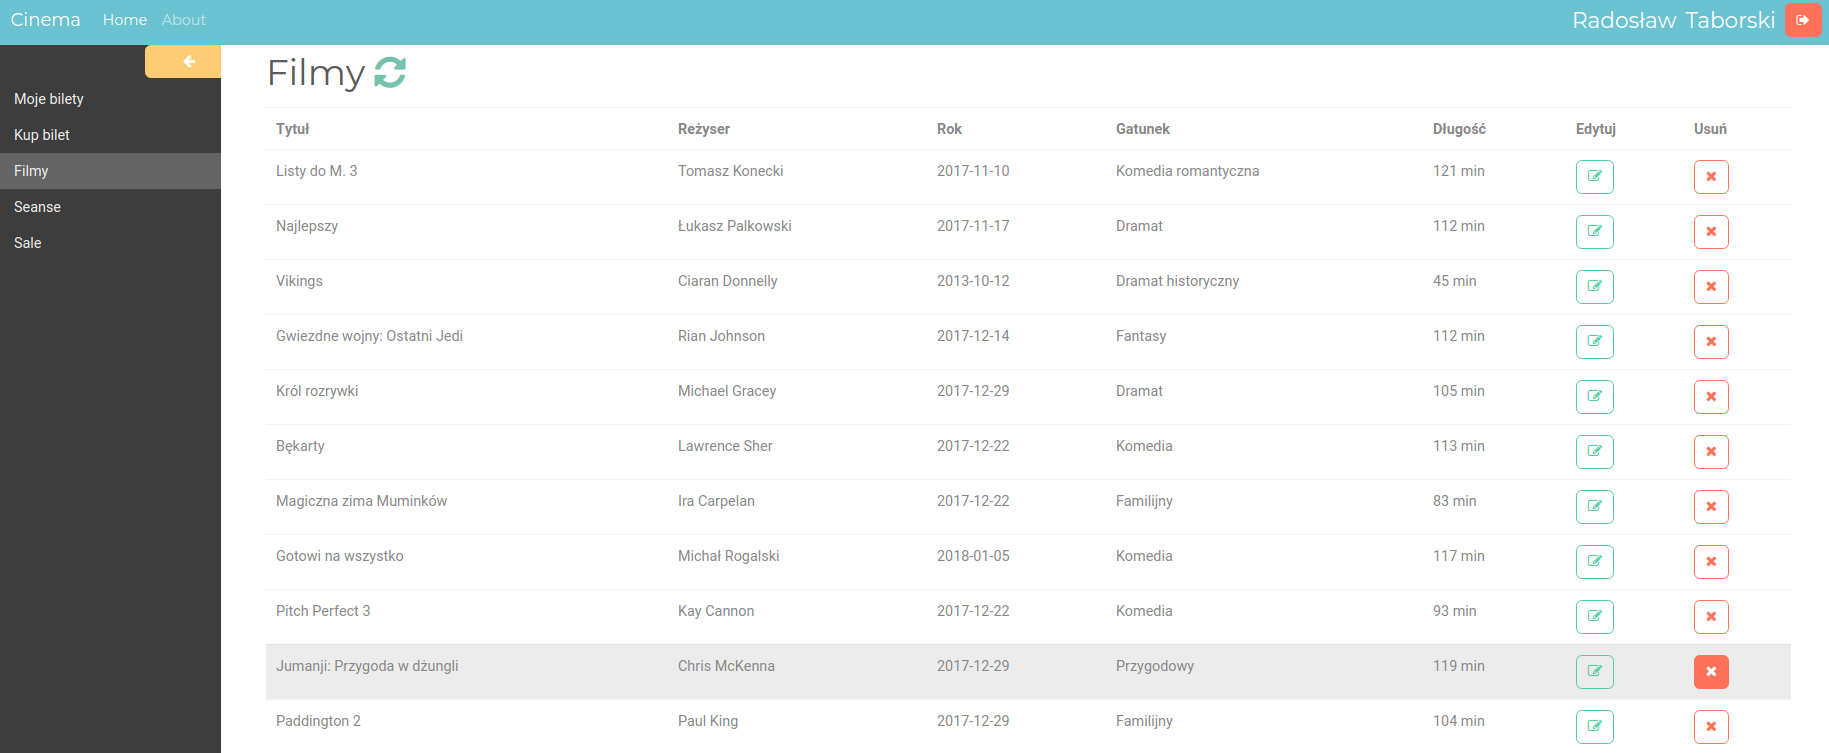
\includegraphics[width=1\linewidth]{rozdzial06/r1.png}
	\caption{Usunięcie filmu poprzez aplikację}
	\label{fig:removeFilm}
\end{figure}

\begin{figure} [H]
	\centering
	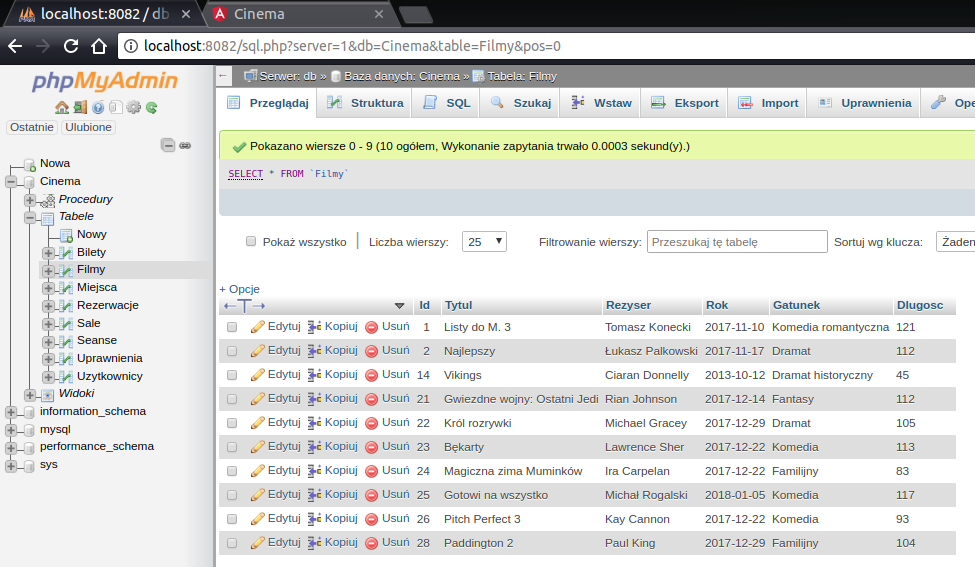
\includegraphics[width=1\linewidth]{rozdzial06/r2.png}
	\caption{Tabela Filmy na węźle \textit{master} o porcie 8082}
	\label{fig:FilmMasterRemove}
\end{figure}

\begin{figure} [H]
	\centering
	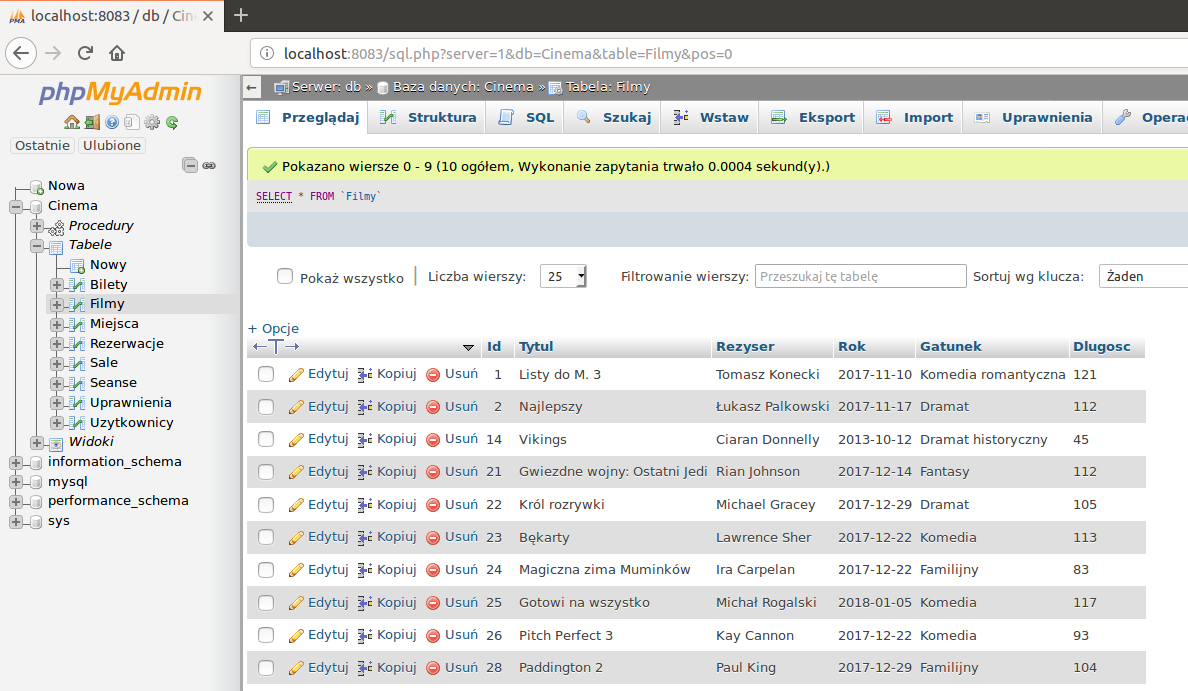
\includegraphics[width=1\linewidth]{rozdzial06/r3.png}
	\caption{Tabela Filmy na węźle \textit{slave1} o porcie 8083}
	\label{fig:FilmSlaveRemove}
\end{figure}

\begin{figure} [H]
	\centering
	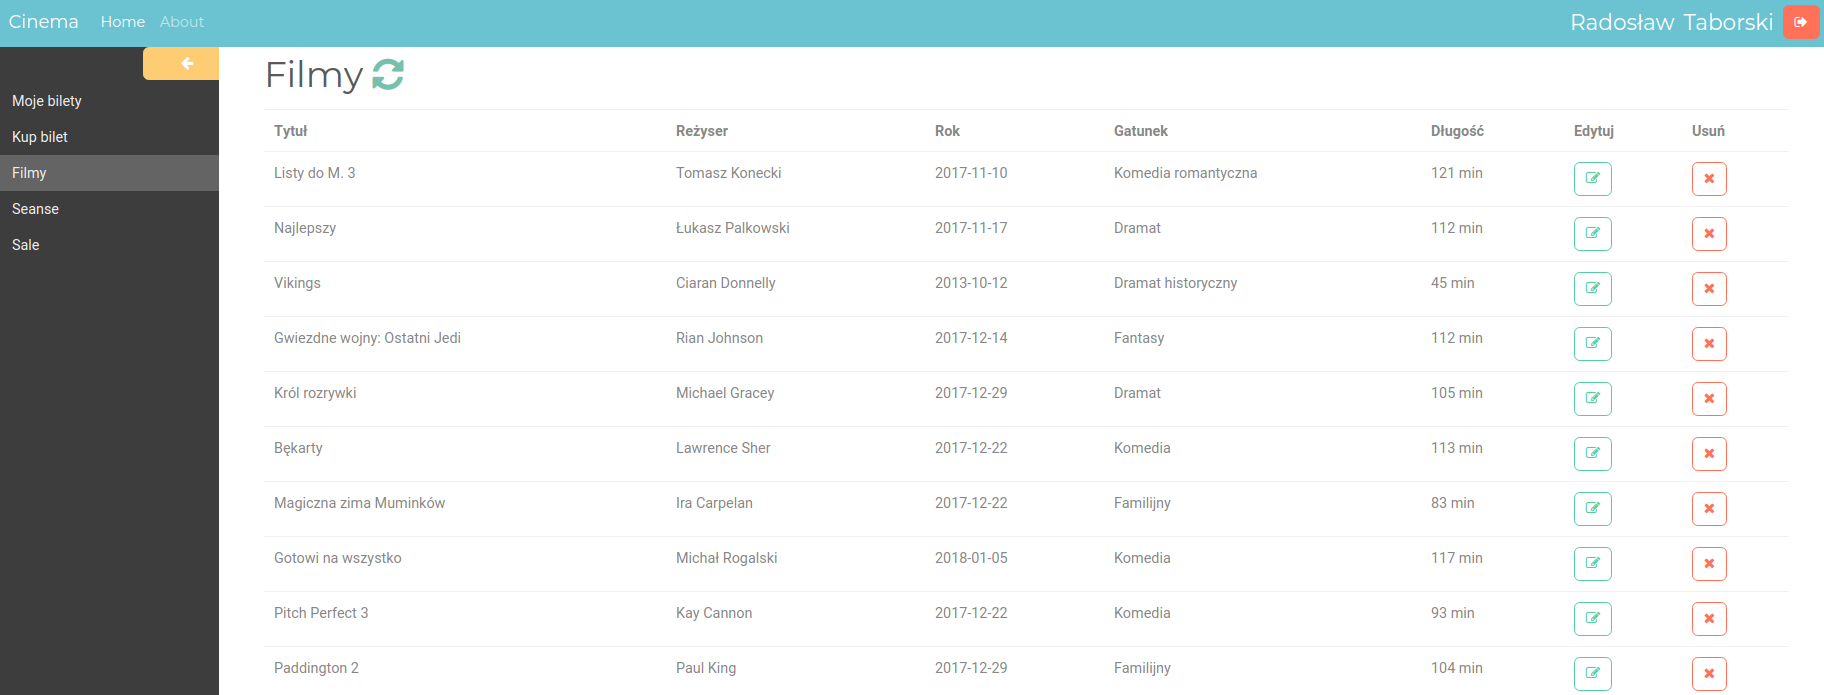
\includegraphics[width=1\linewidth]{rozdzial06/r4.png}
	\caption{Brak usuniętego filmu w aplikacji}
	\label{fig:endRemoveFilm}
\end{figure}




	\chapter{Podsumowanie}

Z powodzeniem zaprojektowano oraz zaimplementowano system obsługi bazodanowej kina.
Wszelkie problemy związane z projektem zostały wyjaśniane i wnikliwie konsultowane z prowadzącym
zajęcia projektowe. Mechanizmy wykorzystywane były skrupulatnie prezentowane na zajęciach,
po drobnych korektach wprowadzono je do systemu bazodanowego tak, aby dążyć do
implementacji pozbawionej błędów formalnych.
System po wykonaniu testów -dodawania tabel, wypełniania ich rekordami działał poprawnie.
Przetestowano moduły zabezpieczeń wspomniane w całym sprawozdaniu projektowym, również
funkcjonowały poprawnie (zabezpieczenia m.in. przed SQLInjection).Projekt całościowo prezentowano
na zajęciach projektowych.\\

W trakcie prac nad realizacją projektu udało się wykorzystać mechanizm replikacji \textit{master-slave} oraz \textit{master-slave} z opóźnieniem. Do ich konfiguracji wykorzystane zostało narzędzie \textit{phpMyAdmin}. \\

Podczas prac nad projektem próbowano wykorzystać jako węzły rozproszonej bazy danych serwery na fizycznych urządzeniach \textit{Raspberry PI}, jednak ilość dostępnych przez nas urządzeń nie pozwalała w pełni pokazać możliwości replikacji w systemie bazodanowym MySQL. Dodatkowo również na system operacyjny \textit{raspbian} nie była dostępna najnowsza wersja MySQL, przez co nie było możliwości m.in. wykonania replikacji z opóźnieniem. Również by replikacja działała wymagane było połączenie internetowe we wszystkich urządzeniach, łącznie z urządzeniem, na którym demonstrowane było działanie. W związku z tym w trakcie prac zrezygnowano z fizycznych urządzeń, a do stworzenia węzłów wykorzystano wirtualne kontenery stworzone w programie \textit{docker}, przez co rozproszona baza danych działa w pełni lokalnie. W każdym kontenerze można było dodać dowolną wersję MySQL oraz \textit{phpMyAdmin}.\\


Interfejs aplikacji bazodanowej jest przejrzysty i intuicyjny, nie jest skomplikowany, dodawanie kolejnych informacji – rekordów nie stanowi żadnych problemów, co jest ważnym atrybutem ze strony spojrzenia konsumenckiego. Implementacja całego projektu pozwoliła na swobodne korzystanie ze strony aktora pracownik jak i aktora klient. Klient posiada inne uprawnienia(na płaszczyźnie szeroko rozumianej rezerwacji seansu w kinie wraz z możliwością opłacenia). Pracownik ma możliwość przeglądania tych rezerwacji, dokonywać ich modyfikacji (np. nagła zmiana repertuaru). Zgodnie z warunkami zadania zaimplementowano możliwość wyświetlania odpowiednich widoków – lista filmów, seansów i biletów.\\

Spełniono wszystkie założenia projektowe postawione przez prowadzącego zajęcia
jak i własne.
	\addcontentsline{toc}{chapter}{Literatura} %utworzenie w spisie treści pozycji Bibliografia
	\pagestyle {empty}

\vspace*{1.3cm}

{\Huge\textbf{Literatura}}

\vspace*{1cm}

\begin{enumerate}[\lbrack 1\rbrack]
	\item Thomson L., Welling L., \textit{PHP i MySQL. Tworzenie stron WWW}, Helion, Gliwice, 2001.
	\item Strona internetowa: \textit{http://wazniak.mimuw.edu.pl/index.php} - systemy rozproszone, zaawansowane
	systemy baz danych, dostęp: 22-11-2017. 
	\item Meloni J. C.,\textit{ PHP-programowanie}, RM, Warszawa, 2001.
	\item Knopczyński P., Talarczyk M., \textit{Duplikacja i replikacja MySQL}, dostęp: 22-11-2017
\end{enumerate}


	
	%\pagestyle {empty}

\vspace*{1.3cm}

{\Huge\textbf{Literatura}}

\vspace*{1cm}

\begin{enumerate}[\lbrack 1\rbrack]
	\item Thomson L., Welling L., \textit{PHP i MySQL. Tworzenie stron WWW}, Helion, Gliwice, 2001.
	\item Strona internetowa: \textit{http://wazniak.mimuw.edu.pl/index.php} - systemy rozproszone, zaawansowane
	systemy baz danych, dostęp: 22-11-2017. 
	\item Meloni J. C.,\textit{ PHP-programowanie}, RM, Warszawa, 2001.
	\item Knopczyński P., Talarczyk M., \textit{Duplikacja i replikacja MySQL}, dostęp: 22-11-2017
\end{enumerate}


	%\bibliography{bibliografia} % wstawia bibliografię korzystając z pliku bibliografia.bib - dotyczy BibTeXa, jeżeli nie korzystamy z BibTeXa należy użyć otoczenia thebibliography
	
\end{document}
